% Options for packages loaded elsewhere
\PassOptionsToPackage{unicode}{hyperref}
\PassOptionsToPackage{hyphens}{url}
%
\documentclass[
]{book}
\usepackage{amsmath,amssymb}
\usepackage{iftex}
\ifPDFTeX
  \usepackage[T1]{fontenc}
  \usepackage[utf8]{inputenc}
  \usepackage{textcomp} % provide euro and other symbols
\else % if luatex or xetex
  \usepackage{unicode-math} % this also loads fontspec
  \defaultfontfeatures{Scale=MatchLowercase}
  \defaultfontfeatures[\rmfamily]{Ligatures=TeX,Scale=1}
\fi
\usepackage{lmodern}
\ifPDFTeX\else
  % xetex/luatex font selection
\fi
% Use upquote if available, for straight quotes in verbatim environments
\IfFileExists{upquote.sty}{\usepackage{upquote}}{}
\IfFileExists{microtype.sty}{% use microtype if available
  \usepackage[]{microtype}
  \UseMicrotypeSet[protrusion]{basicmath} % disable protrusion for tt fonts
}{}
\makeatletter
\@ifundefined{KOMAClassName}{% if non-KOMA class
  \IfFileExists{parskip.sty}{%
    \usepackage{parskip}
  }{% else
    \setlength{\parindent}{0pt}
    \setlength{\parskip}{6pt plus 2pt minus 1pt}}
}{% if KOMA class
  \KOMAoptions{parskip=half}}
\makeatother
\usepackage{xcolor}
\usepackage{color}
\usepackage{fancyvrb}
\newcommand{\VerbBar}{|}
\newcommand{\VERB}{\Verb[commandchars=\\\{\}]}
\DefineVerbatimEnvironment{Highlighting}{Verbatim}{commandchars=\\\{\}}
% Add ',fontsize=\small' for more characters per line
\usepackage{framed}
\definecolor{shadecolor}{RGB}{248,248,248}
\newenvironment{Shaded}{\begin{snugshade}}{\end{snugshade}}
\newcommand{\AlertTok}[1]{\textcolor[rgb]{0.94,0.16,0.16}{#1}}
\newcommand{\AnnotationTok}[1]{\textcolor[rgb]{0.56,0.35,0.01}{\textbf{\textit{#1}}}}
\newcommand{\AttributeTok}[1]{\textcolor[rgb]{0.13,0.29,0.53}{#1}}
\newcommand{\BaseNTok}[1]{\textcolor[rgb]{0.00,0.00,0.81}{#1}}
\newcommand{\BuiltInTok}[1]{#1}
\newcommand{\CharTok}[1]{\textcolor[rgb]{0.31,0.60,0.02}{#1}}
\newcommand{\CommentTok}[1]{\textcolor[rgb]{0.56,0.35,0.01}{\textit{#1}}}
\newcommand{\CommentVarTok}[1]{\textcolor[rgb]{0.56,0.35,0.01}{\textbf{\textit{#1}}}}
\newcommand{\ConstantTok}[1]{\textcolor[rgb]{0.56,0.35,0.01}{#1}}
\newcommand{\ControlFlowTok}[1]{\textcolor[rgb]{0.13,0.29,0.53}{\textbf{#1}}}
\newcommand{\DataTypeTok}[1]{\textcolor[rgb]{0.13,0.29,0.53}{#1}}
\newcommand{\DecValTok}[1]{\textcolor[rgb]{0.00,0.00,0.81}{#1}}
\newcommand{\DocumentationTok}[1]{\textcolor[rgb]{0.56,0.35,0.01}{\textbf{\textit{#1}}}}
\newcommand{\ErrorTok}[1]{\textcolor[rgb]{0.64,0.00,0.00}{\textbf{#1}}}
\newcommand{\ExtensionTok}[1]{#1}
\newcommand{\FloatTok}[1]{\textcolor[rgb]{0.00,0.00,0.81}{#1}}
\newcommand{\FunctionTok}[1]{\textcolor[rgb]{0.13,0.29,0.53}{\textbf{#1}}}
\newcommand{\ImportTok}[1]{#1}
\newcommand{\InformationTok}[1]{\textcolor[rgb]{0.56,0.35,0.01}{\textbf{\textit{#1}}}}
\newcommand{\KeywordTok}[1]{\textcolor[rgb]{0.13,0.29,0.53}{\textbf{#1}}}
\newcommand{\NormalTok}[1]{#1}
\newcommand{\OperatorTok}[1]{\textcolor[rgb]{0.81,0.36,0.00}{\textbf{#1}}}
\newcommand{\OtherTok}[1]{\textcolor[rgb]{0.56,0.35,0.01}{#1}}
\newcommand{\PreprocessorTok}[1]{\textcolor[rgb]{0.56,0.35,0.01}{\textit{#1}}}
\newcommand{\RegionMarkerTok}[1]{#1}
\newcommand{\SpecialCharTok}[1]{\textcolor[rgb]{0.81,0.36,0.00}{\textbf{#1}}}
\newcommand{\SpecialStringTok}[1]{\textcolor[rgb]{0.31,0.60,0.02}{#1}}
\newcommand{\StringTok}[1]{\textcolor[rgb]{0.31,0.60,0.02}{#1}}
\newcommand{\VariableTok}[1]{\textcolor[rgb]{0.00,0.00,0.00}{#1}}
\newcommand{\VerbatimStringTok}[1]{\textcolor[rgb]{0.31,0.60,0.02}{#1}}
\newcommand{\WarningTok}[1]{\textcolor[rgb]{0.56,0.35,0.01}{\textbf{\textit{#1}}}}
\usepackage{longtable,booktabs,array}
\usepackage{calc} % for calculating minipage widths
% Correct order of tables after \paragraph or \subparagraph
\usepackage{etoolbox}
\makeatletter
\patchcmd\longtable{\par}{\if@noskipsec\mbox{}\fi\par}{}{}
\makeatother
% Allow footnotes in longtable head/foot
\IfFileExists{footnotehyper.sty}{\usepackage{footnotehyper}}{\usepackage{footnote}}
\makesavenoteenv{longtable}
\usepackage{graphicx}
\makeatletter
\def\maxwidth{\ifdim\Gin@nat@width>\linewidth\linewidth\else\Gin@nat@width\fi}
\def\maxheight{\ifdim\Gin@nat@height>\textheight\textheight\else\Gin@nat@height\fi}
\makeatother
% Scale images if necessary, so that they will not overflow the page
% margins by default, and it is still possible to overwrite the defaults
% using explicit options in \includegraphics[width, height, ...]{}
\setkeys{Gin}{width=\maxwidth,height=\maxheight,keepaspectratio}
% Set default figure placement to htbp
\makeatletter
\def\fps@figure{htbp}
\makeatother
\setlength{\emergencystretch}{3em} % prevent overfull lines
\providecommand{\tightlist}{%
  \setlength{\itemsep}{0pt}\setlength{\parskip}{0pt}}
\setcounter{secnumdepth}{5}
\usepackage{booktabs}
\usepackage{amsthm}
\makeatletter
\def\thm@space@setup{%
  \thm@preskip=8pt plus 2pt minus 4pt
  \thm@postskip=\thm@preskip
}
\makeatother
\ifLuaTeX
  \usepackage{selnolig}  % disable illegal ligatures
\fi
\usepackage[]{natbib}
\bibliographystyle{apalike}
\IfFileExists{bookmark.sty}{\usepackage{bookmark}}{\usepackage{hyperref}}
\IfFileExists{xurl.sty}{\usepackage{xurl}}{} % add URL line breaks if available
\urlstyle{same}
\hypersetup{
  pdftitle={MODELACIÓN DEL PRECIO PARA LA COMPRA Y VENTA DE ACEITE DE SOYA},
  pdfauthor={Nidia Munevar - Leonardo Palacios},
  hidelinks,
  pdfcreator={LaTeX via pandoc}}

\title{MODELACIÓN DEL PRECIO PARA LA COMPRA Y VENTA DE ACEITE DE SOYA}
\author{Nidia Munevar - Leonardo Palacios}
\date{2023-10-02}

\begin{document}
\maketitle

{
\setcounter{tocdepth}{1}
\tableofcontents
}
\hypertarget{resumen}{%
\chapter{Resumen}\label{resumen}}

El proyecto aplicado a realizar es la modelación del precio para la compra y venta de aceite de soya.

\hypertarget{introduccion}{%
\chapter{Introduccion}\label{introduccion}}

En el mercado de venta y compra de materias primas agrícolas intervienen diferentes actores, los precios son públicos y son afectados por diferentes variables tales como el precio del petróleo, la tasa de cambio, el clima entre otros elementos. La necesidad de los actores es mejorar sus decisiones y de esta forma su rentabilidad, los precios de las materias primas afectan directamente al mercado y a los precios de los bienes producidos a partir de estas, es decir estos valores terminan impactando al comprador final.

\hypertarget{justificacion}{%
\chapter{Justificacion}\label{justificacion}}

El proyecto está planteado ante una necesidad de los actores que requieren mejorar sus decisiones y de esta forma su rentabilidad. Los precios de las materias primas afectan directamente al mercado y a los precios de los bienes producidos a partir de estas materias, es decir estos valores terminan impactando al comprador final.

\hypertarget{serie-de-tiempo}{%
\chapter{Serie de Tiempo}\label{serie-de-tiempo}}

\begin{Shaded}
\begin{Highlighting}[]
\CommentTok{\# Cargar la biblioteca quantmod}
\FunctionTok{library}\NormalTok{(quantmod)}
\end{Highlighting}
\end{Shaded}

\begin{verbatim}
## Loading required package: xts
\end{verbatim}

\begin{verbatim}
## Loading required package: zoo
\end{verbatim}

\begin{verbatim}
## 
## Attaching package: 'zoo'
\end{verbatim}

\begin{verbatim}
## The following objects are masked from 'package:base':
## 
##     as.Date, as.Date.numeric
\end{verbatim}

\begin{verbatim}
## Loading required package: TTR
\end{verbatim}

\begin{verbatim}
## Registered S3 method overwritten by 'quantmod':
##   method            from
##   as.zoo.data.frame zoo
\end{verbatim}

\begin{Shaded}
\begin{Highlighting}[]
\CommentTok{\# Especificar el símbolo para futuros de soja}
\NormalTok{symbol }\OtherTok{\textless{}{-}} \StringTok{"ZS=F"}

\CommentTok{\# Descargar los datos históricos desde el 1 de enero de 2010 hasta}
\CommentTok{\# hoy}
\FunctionTok{getSymbols}\NormalTok{(symbol, }\AttributeTok{from =} \StringTok{"2010{-}01{-}01"}\NormalTok{, }\AttributeTok{to =} \FunctionTok{Sys.Date}\NormalTok{(), }
\AttributeTok{auto.assign =} \ConstantTok{TRUE}\NormalTok{)}
\end{Highlighting}
\end{Shaded}

\begin{verbatim}
## [1] "ZS=F"
\end{verbatim}

\begin{Shaded}
\begin{Highlighting}[]
\CommentTok{\# Crear un data frame con la serie de tiempo}
\NormalTok{soybean\_data }\OtherTok{\textless{}{-}} \FunctionTok{data.frame}\NormalTok{(}\AttributeTok{Date =} \FunctionTok{index}\NormalTok{(}\FunctionTok{get}\NormalTok{(symbol)), }
                           \AttributeTok{Open =} \FunctionTok{Op}\NormalTok{(}\FunctionTok{get}\NormalTok{(symbol)),}
                           \AttributeTok{High =} \FunctionTok{Hi}\NormalTok{(}\FunctionTok{get}\NormalTok{(symbol)),}
                           \AttributeTok{Low =} \FunctionTok{Lo}\NormalTok{(}\FunctionTok{get}\NormalTok{(symbol)),}
                           \AttributeTok{Close =} \FunctionTok{Cl}\NormalTok{(}\FunctionTok{get}\NormalTok{(symbol)),}
                           \AttributeTok{Volume =} \FunctionTok{Vo}\NormalTok{(}\FunctionTok{get}\NormalTok{(symbol))}
\NormalTok{                           )}

\CommentTok{\# Eliminar filas con valores NA}
\NormalTok{soybean\_data }\OtherTok{\textless{}{-}} \FunctionTok{na.omit}\NormalTok{(soybean\_data)}

\CommentTok{\# Muestra los primeros registros del data frame}
\FunctionTok{head}\NormalTok{(soybean\_data)}
\end{Highlighting}
\end{Shaded}

\begin{verbatim}
##                  Date ZS.F.Open ZS.F.High ZS.F.Low ZS.F.Close ZS.F.Volume
## 2010-01-04 2010-01-04   1043.00   1065.50  1041.25    1049.50       25947
## 2010-01-05 2010-01-05   1047.00   1056.00  1042.00    1052.25       21073
## 2010-01-06 2010-01-06   1050.00   1058.50  1042.75    1050.50       17567
## 2010-01-07 2010-01-07   1050.50   1052.00  1016.50    1017.75       11750
## 2010-01-08 2010-01-08   1018.25   1018.25  1005.00    1013.00       11750
## 2010-01-11 2010-01-11   1014.00   1022.00   997.50    1001.75       11750
\end{verbatim}

\begin{Shaded}
\begin{Highlighting}[]
\FunctionTok{class}\NormalTok{(soybean\_data)}
\end{Highlighting}
\end{Shaded}

\begin{verbatim}
## [1] "data.frame"
\end{verbatim}

\begin{Shaded}
\begin{Highlighting}[]
\CommentTok{\# Cargar la biblioteca xts}
\FunctionTok{library}\NormalTok{(xts)}

\CommentTok{\# Crear una serie de tiempo xts a partir del data frame soybean\_data}
\NormalTok{soybean\_xts }\OtherTok{\textless{}{-}} \FunctionTok{xts}\NormalTok{(soybean\_data[, }\SpecialCharTok{{-}}\DecValTok{1}\NormalTok{], }\AttributeTok{order.by =}\NormalTok{ soybean\_data}\SpecialCharTok{$}\NormalTok{Date)}

\CommentTok{\# Verificar la serie de tiempo}
\FunctionTok{head}\NormalTok{(soybean\_xts)}
\end{Highlighting}
\end{Shaded}

\begin{verbatim}
##            ZS.F.Open ZS.F.High ZS.F.Low ZS.F.Close ZS.F.Volume
## 2010-01-04   1043.00   1065.50  1041.25    1049.50       25947
## 2010-01-05   1047.00   1056.00  1042.00    1052.25       21073
## 2010-01-06   1050.00   1058.50  1042.75    1050.50       17567
## 2010-01-07   1050.50   1052.00  1016.50    1017.75       11750
## 2010-01-08   1018.25   1018.25  1005.00    1013.00       11750
## 2010-01-11   1014.00   1022.00   997.50    1001.75       11750
\end{verbatim}

\begin{Shaded}
\begin{Highlighting}[]
\FunctionTok{class}\NormalTok{(soybean\_xts)}
\end{Highlighting}
\end{Shaded}

\begin{verbatim}
## [1] "xts" "zoo"
\end{verbatim}

\hypertarget{analisis-exploratorio}{%
\chapter{Analisis Exploratorio}\label{analisis-exploratorio}}

\begin{Shaded}
\begin{Highlighting}[]
\CommentTok{\# Cargar la biblioteca quantmod}
\FunctionTok{library}\NormalTok{(quantmod)}

\CommentTok{\# Especificar el símbolo para futuros de soja}
\NormalTok{symbol }\OtherTok{\textless{}{-}} \StringTok{"ZS=F"}

\CommentTok{\# Descargar los datos históricos desde el 1 de enero de 2010 hasta}
\CommentTok{\# hoy}
\FunctionTok{getSymbols}\NormalTok{(symbol, }\AttributeTok{from =} \StringTok{"2010{-}01{-}01"}\NormalTok{, }\AttributeTok{to =} \FunctionTok{Sys.Date}\NormalTok{(), }
\AttributeTok{auto.assign =} \ConstantTok{TRUE}\NormalTok{)}
\end{Highlighting}
\end{Shaded}

\begin{verbatim}
## [1] "ZS=F"
\end{verbatim}

\begin{Shaded}
\begin{Highlighting}[]
\CommentTok{\# Crear un data frame con la serie de tiempo}
\NormalTok{soybean\_data }\OtherTok{\textless{}{-}} \FunctionTok{data.frame}\NormalTok{(}\AttributeTok{Date =} \FunctionTok{index}\NormalTok{(}\FunctionTok{get}\NormalTok{(symbol)), }
                           \AttributeTok{Open =} \FunctionTok{Op}\NormalTok{(}\FunctionTok{get}\NormalTok{(symbol)),}
                           \AttributeTok{High =} \FunctionTok{Hi}\NormalTok{(}\FunctionTok{get}\NormalTok{(symbol)),}
                           \AttributeTok{Low =} \FunctionTok{Lo}\NormalTok{(}\FunctionTok{get}\NormalTok{(symbol)),}
                           \AttributeTok{Close =} \FunctionTok{Cl}\NormalTok{(}\FunctionTok{get}\NormalTok{(symbol)),}
                           \AttributeTok{Volume =} \FunctionTok{Vo}\NormalTok{(}\FunctionTok{get}\NormalTok{(symbol))}
\NormalTok{)}

\CommentTok{\# Eliminar filas con valores NA}
\NormalTok{soybean\_data }\OtherTok{\textless{}{-}} \FunctionTok{na.omit}\NormalTok{(soybean\_data)}


\FunctionTok{head}\NormalTok{(soybean\_data)}
\end{Highlighting}
\end{Shaded}

\begin{verbatim}
##                  Date ZS.F.Open ZS.F.High ZS.F.Low ZS.F.Close ZS.F.Volume
## 2010-01-04 2010-01-04   1043.00   1065.50  1041.25    1049.50       25947
## 2010-01-05 2010-01-05   1047.00   1056.00  1042.00    1052.25       21073
## 2010-01-06 2010-01-06   1050.00   1058.50  1042.75    1050.50       17567
## 2010-01-07 2010-01-07   1050.50   1052.00  1016.50    1017.75       11750
## 2010-01-08 2010-01-08   1018.25   1018.25  1005.00    1013.00       11750
## 2010-01-11 2010-01-11   1014.00   1022.00   997.50    1001.75       11750
\end{verbatim}

\begin{Shaded}
\begin{Highlighting}[]
\CommentTok{\# Cargar la biblioteca xts}
\FunctionTok{library}\NormalTok{(xts)}

\CommentTok{\# Crear una serie de tiempo xts a partir del data frame soybean\_data}
\NormalTok{soybean\_xts }\OtherTok{\textless{}{-}} \FunctionTok{xts}\NormalTok{(soybean\_data[, }\SpecialCharTok{{-}}\DecValTok{1}\NormalTok{], }\AttributeTok{order.by =}\NormalTok{ soybean\_data}\SpecialCharTok{$}\NormalTok{Date)}

\CommentTok{\# Verificar la serie de tiempo}
\FunctionTok{head}\NormalTok{(soybean\_xts)}
\end{Highlighting}
\end{Shaded}

\begin{verbatim}
##            ZS.F.Open ZS.F.High ZS.F.Low ZS.F.Close ZS.F.Volume
## 2010-01-04   1043.00   1065.50  1041.25    1049.50       25947
## 2010-01-05   1047.00   1056.00  1042.00    1052.25       21073
## 2010-01-06   1050.00   1058.50  1042.75    1050.50       17567
## 2010-01-07   1050.50   1052.00  1016.50    1017.75       11750
## 2010-01-08   1018.25   1018.25  1005.00    1013.00       11750
## 2010-01-11   1014.00   1022.00   997.50    1001.75       11750
\end{verbatim}

\begin{Shaded}
\begin{Highlighting}[]
\FunctionTok{class}\NormalTok{(soybean\_xts)}
\end{Highlighting}
\end{Shaded}

\begin{verbatim}
## [1] "xts" "zoo"
\end{verbatim}

\begin{Shaded}
\begin{Highlighting}[]
\CommentTok{\# Acceder a la columna "ZS.F.Close" en soybean\_xts}
\NormalTok{close\_prices }\OtherTok{\textless{}{-}}\NormalTok{ soybean\_xts[, }\StringTok{"ZS.F.Close"}\NormalTok{]}

\CommentTok{\# Imprimir las primeras filas de la columna Close}
\FunctionTok{print}\NormalTok{(}\FunctionTok{head}\NormalTok{(close\_prices))}
\end{Highlighting}
\end{Shaded}

\begin{verbatim}
##            ZS.F.Close
## 2010-01-04    1049.50
## 2010-01-05    1052.25
## 2010-01-06    1050.50
## 2010-01-07    1017.75
## 2010-01-08    1013.00
## 2010-01-11    1001.75
\end{verbatim}

\begin{Shaded}
\begin{Highlighting}[]
\FunctionTok{head}\NormalTok{(soybean\_xts)}
\end{Highlighting}
\end{Shaded}

\begin{verbatim}
##            ZS.F.Open ZS.F.High ZS.F.Low ZS.F.Close ZS.F.Volume
## 2010-01-04   1043.00   1065.50  1041.25    1049.50       25947
## 2010-01-05   1047.00   1056.00  1042.00    1052.25       21073
## 2010-01-06   1050.00   1058.50  1042.75    1050.50       17567
## 2010-01-07   1050.50   1052.00  1016.50    1017.75       11750
## 2010-01-08   1018.25   1018.25  1005.00    1013.00       11750
## 2010-01-11   1014.00   1022.00   997.50    1001.75       11750
\end{verbatim}

\begin{Shaded}
\begin{Highlighting}[]
\CommentTok{\# Cargar la biblioteca ggplot2 para hacer gráficos}
\FunctionTok{library}\NormalTok{(ggplot2)}
\end{Highlighting}
\end{Shaded}

\begin{verbatim}
## Warning: package 'ggplot2' was built under R version 4.2.3
\end{verbatim}

\begin{Shaded}
\begin{Highlighting}[]
\CommentTok{\# Crear un gráfico de serie de tiempo}
\FunctionTok{ggplot}\NormalTok{(}\AttributeTok{data =} \ConstantTok{NULL}\NormalTok{, }\FunctionTok{aes}\NormalTok{(}\AttributeTok{x =} \FunctionTok{index}\NormalTok{(close\_prices), }\AttributeTok{y =}\NormalTok{ close\_prices)) }\SpecialCharTok{+}
  \FunctionTok{geom\_line}\NormalTok{(}\AttributeTok{color =} \StringTok{"blue"}\NormalTok{) }\SpecialCharTok{+}
  \FunctionTok{labs}\NormalTok{(}\AttributeTok{x =} \StringTok{"Fecha"}\NormalTok{, }\AttributeTok{y =} \StringTok{"Precio de Cierre"}\NormalTok{, }\AttributeTok{title =} \StringTok{"Serie de }
\StringTok{\# Tiempo de Futuros de Soja"}\NormalTok{) }\SpecialCharTok{+}
  \FunctionTok{theme\_minimal}\NormalTok{()}
\end{Highlighting}
\end{Shaded}

\begin{verbatim}
## Don't know how to automatically pick scale for object of type <xts/zoo>.
## Defaulting to continuous.
\end{verbatim}

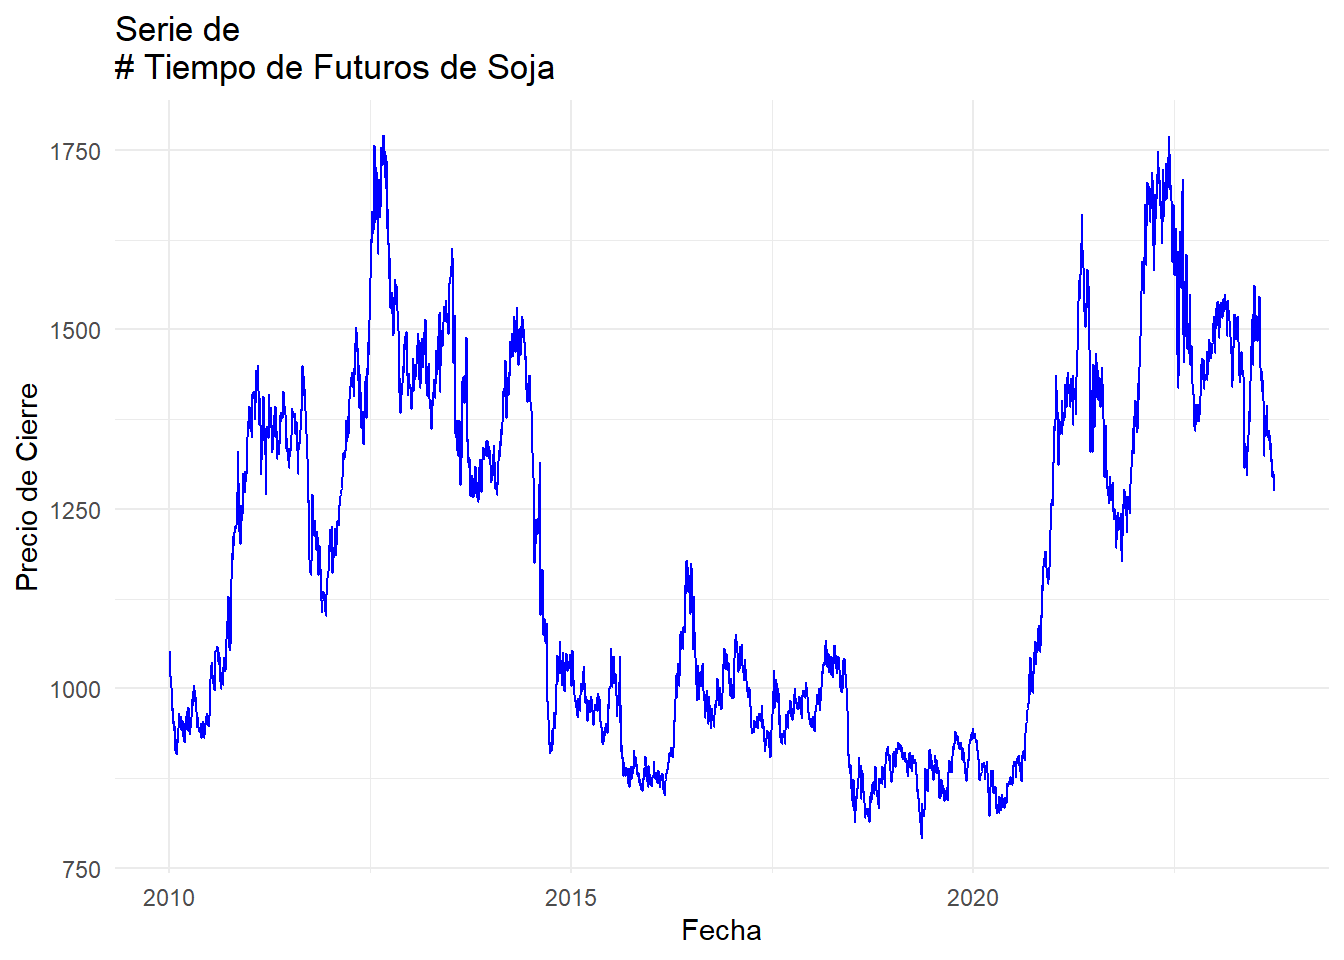
\includegraphics{bookdown-demo_files/figure-latex/unnamed-chunk-10-1.pdf}

\hypertarget{promedio-movil}{%
\chapter{Promedio Movil}\label{promedio-movil}}

Cuando aplicamos un promedio móvil a una serie de tiempo, cada punto de la serie transformada (promediada) es el promedio de un número determinado de puntos anteriores, actuales y futuros de la serie original. Este número de puntos que decides promediar se llama ``ventana'' del promedio móvil.

\begin{Shaded}
\begin{Highlighting}[]
\CommentTok{\# Cargar la biblioteca quantmod}
\FunctionTok{library}\NormalTok{(quantmod)}

\CommentTok{\# Especificar el símbolo para futuros de soja}
\NormalTok{symbol }\OtherTok{\textless{}{-}} \StringTok{"ZS=F"}

\CommentTok{\# Descargar los datos históricos desde el 1 de enero de 2010 }
\CommentTok{\# hasta hoy}
\FunctionTok{getSymbols}\NormalTok{(symbol, }\AttributeTok{from =} \StringTok{"2010{-}01{-}01"}\NormalTok{, }\AttributeTok{to =} \FunctionTok{Sys.Date}\NormalTok{(), }
\AttributeTok{auto.assign =} \ConstantTok{TRUE}\NormalTok{)}
\end{Highlighting}
\end{Shaded}

\begin{verbatim}
## Warning: ZS=F contains missing values. Some functions will not work if objects
## contain missing values in the middle of the series. Consider using na.omit(),
## na.approx(), na.fill(), etc to remove or replace them.
\end{verbatim}

\begin{verbatim}
## [1] "ZS=F"
\end{verbatim}

\begin{Shaded}
\begin{Highlighting}[]
\CommentTok{\# Crear un data frame con la serie de tiempo}
\NormalTok{soybean\_data }\OtherTok{\textless{}{-}} \FunctionTok{data.frame}\NormalTok{(}\AttributeTok{Date =} \FunctionTok{index}\NormalTok{(}\FunctionTok{get}\NormalTok{(symbol)), }
                           \AttributeTok{Open =} \FunctionTok{Op}\NormalTok{(}\FunctionTok{get}\NormalTok{(symbol)),}
                           \AttributeTok{High =} \FunctionTok{Hi}\NormalTok{(}\FunctionTok{get}\NormalTok{(symbol)),}
                           \AttributeTok{Low =} \FunctionTok{Lo}\NormalTok{(}\FunctionTok{get}\NormalTok{(symbol)),}
                           \AttributeTok{Close =} \FunctionTok{Cl}\NormalTok{(}\FunctionTok{get}\NormalTok{(symbol)),}
                           \AttributeTok{Volume =} \FunctionTok{Vo}\NormalTok{(}\FunctionTok{get}\NormalTok{(symbol))}
\NormalTok{                           )}

\CommentTok{\# Eliminar filas con valores NA}
\NormalTok{soybean\_data }\OtherTok{\textless{}{-}} \FunctionTok{na.omit}\NormalTok{(soybean\_data)}

\CommentTok{\# Muestra los primeros registros del data frame}
\CommentTok{\# head(soybean\_data)}
\end{Highlighting}
\end{Shaded}

\begin{Shaded}
\begin{Highlighting}[]
\CommentTok{\# Cargar la biblioteca xts}
\FunctionTok{library}\NormalTok{(xts)}

\CommentTok{\# Crear una serie de tiempo xts a partir del data frame soybean\_data}
\NormalTok{soybean\_xts }\OtherTok{\textless{}{-}} \FunctionTok{xts}\NormalTok{(soybean\_data[, }\SpecialCharTok{{-}}\DecValTok{1}\NormalTok{], }\AttributeTok{order.by =}\NormalTok{ soybean\_data}\SpecialCharTok{$}\NormalTok{Date)}

\CommentTok{\# Verificar la serie de tiempo}
\CommentTok{\# head(soybean\_xts)}
\end{Highlighting}
\end{Shaded}

\begin{Shaded}
\begin{Highlighting}[]
\FunctionTok{library}\NormalTok{(ggplot2)}
\FunctionTok{library}\NormalTok{(TTR)}
\FunctionTok{library}\NormalTok{(scales)}
\end{Highlighting}
\end{Shaded}

\begin{verbatim}
## Warning: package 'scales' was built under R version 4.2.3
\end{verbatim}

\begin{Shaded}
\begin{Highlighting}[]
\CommentTok{\# Convertir el objeto xts a data.frame}
\NormalTok{soybean\_df }\OtherTok{\textless{}{-}} \FunctionTok{as.data.frame}\NormalTok{(soybean\_xts)}
\NormalTok{soybean\_df}\SpecialCharTok{$}\NormalTok{Date }\OtherTok{\textless{}{-}} \FunctionTok{index}\NormalTok{(soybean\_xts)}

\CommentTok{\# Calcular SMA\_200 y SMA\_500}
\NormalTok{soybean\_df}\SpecialCharTok{$}\NormalTok{SMA\_200 }\OtherTok{\textless{}{-}} \FunctionTok{SMA}\NormalTok{(soybean\_df}\SpecialCharTok{$}\NormalTok{ZS.F.Close, }\AttributeTok{n =} \DecValTok{200}\NormalTok{)}
\NormalTok{soybean\_df}\SpecialCharTok{$}\NormalTok{SMA\_500 }\OtherTok{\textless{}{-}} \FunctionTok{SMA}\NormalTok{(soybean\_df}\SpecialCharTok{$}\NormalTok{ZS.F.Close, }\AttributeTok{n =} \DecValTok{500}\NormalTok{)}

\CommentTok{\# Usar ggplot2 para visualizar los datos}
\FunctionTok{ggplot}\NormalTok{(soybean\_df, }\FunctionTok{aes}\NormalTok{(}\AttributeTok{x =}\NormalTok{ Date)) }\SpecialCharTok{+}
  \FunctionTok{geom\_line}\NormalTok{(}\FunctionTok{aes}\NormalTok{(}\AttributeTok{y =}\NormalTok{ ZS.F.Close, }\AttributeTok{color =} \StringTok{\textquotesingle{}Precio de Cierre\textquotesingle{}}\NormalTok{),}
  \AttributeTok{alpha =} \FloatTok{0.75}\NormalTok{) }\SpecialCharTok{+}
  \FunctionTok{geom\_line}\NormalTok{(}\FunctionTok{aes}\NormalTok{(}\AttributeTok{y =}\NormalTok{ SMA\_200, }\AttributeTok{color =} \StringTok{\textquotesingle{}Promedio Móvil 200\textquotesingle{}}\NormalTok{), }
  \AttributeTok{size =} \DecValTok{1}\NormalTok{, }\AttributeTok{na.rm =} \ConstantTok{TRUE}\NormalTok{) }\SpecialCharTok{+}
  \FunctionTok{geom\_line}\NormalTok{(}\FunctionTok{aes}\NormalTok{(}\AttributeTok{y =}\NormalTok{ SMA\_500, }\AttributeTok{color =} \StringTok{\textquotesingle{}Promedio Móvil 500\textquotesingle{}}\NormalTok{), }
  \AttributeTok{size =} \DecValTok{1}\NormalTok{, }\AttributeTok{na.rm =} \ConstantTok{TRUE}\NormalTok{) }\SpecialCharTok{+}
  \FunctionTok{theme\_minimal}\NormalTok{(}\AttributeTok{base\_size =} \DecValTok{15}\NormalTok{) }\SpecialCharTok{+}
  \FunctionTok{labs}\NormalTok{(}\AttributeTok{title =} \StringTok{\textquotesingle{}Serie de Tiempo de Futuros de Soja\textquotesingle{}}\NormalTok{,}
       \AttributeTok{subtitle =} \StringTok{\textquotesingle{}Con Promedios Móviles de 200 y 500 Días\textquotesingle{}}\NormalTok{,}
       \AttributeTok{y =} \StringTok{\textquotesingle{}Precio de Cierre\textquotesingle{}}\NormalTok{) }\SpecialCharTok{+}
  \FunctionTok{theme}\NormalTok{(}\AttributeTok{axis.title.x =} \FunctionTok{element\_blank}\NormalTok{(),}
        \AttributeTok{axis.text.x =} \FunctionTok{element\_text}\NormalTok{(}\AttributeTok{size =} \DecValTok{10}\NormalTok{, }\AttributeTok{angle =} \DecValTok{90}\NormalTok{, }
        \AttributeTok{vjust =} \FloatTok{0.5}\NormalTok{),}
        \AttributeTok{plot.title =} \FunctionTok{element\_text}\NormalTok{(}\AttributeTok{hjust =} \FloatTok{0.5}\NormalTok{),}
        \AttributeTok{plot.subtitle =} \FunctionTok{element\_text}\NormalTok{(}\AttributeTok{hjust =} \FloatTok{0.5}\NormalTok{),}
        \AttributeTok{legend.position =} \StringTok{"bottom"}\NormalTok{) }\SpecialCharTok{+}
  \FunctionTok{scale\_x\_date}\NormalTok{(}\AttributeTok{date\_breaks =} \StringTok{"1 year"}\NormalTok{, }\AttributeTok{date\_labels =} \StringTok{"\%Y"}\NormalTok{) }\SpecialCharTok{+}
  \FunctionTok{scale\_y\_continuous}\NormalTok{(}\AttributeTok{labels =} \FunctionTok{dollar\_format}\NormalTok{()) }\SpecialCharTok{+}
  \FunctionTok{scale\_color\_manual}\NormalTok{(}\AttributeTok{values =} \FunctionTok{c}\NormalTok{(}\StringTok{\textquotesingle{}Precio de Cierre\textquotesingle{}} \OtherTok{=} \StringTok{\textquotesingle{}blue\textquotesingle{}}\NormalTok{,}
  \StringTok{\textquotesingle{}Promedio Móvil 200\textquotesingle{}} \OtherTok{=} \StringTok{\textquotesingle{}red\textquotesingle{}}\NormalTok{, }\StringTok{\textquotesingle{}Promedio Móvil 500\textquotesingle{}} \OtherTok{=} \StringTok{\textquotesingle{}green\textquotesingle{}}\NormalTok{),}
                     \AttributeTok{name =} \StringTok{""}\NormalTok{)}
\end{Highlighting}
\end{Shaded}

\begin{verbatim}
## Warning: Using `size` aesthetic for lines was deprecated in ggplot2 3.4.0.
## i Please use `linewidth` instead.
## This warning is displayed once every 8 hours.
## Call `lifecycle::last_lifecycle_warnings()` to see where this warning was
## generated.
\end{verbatim}

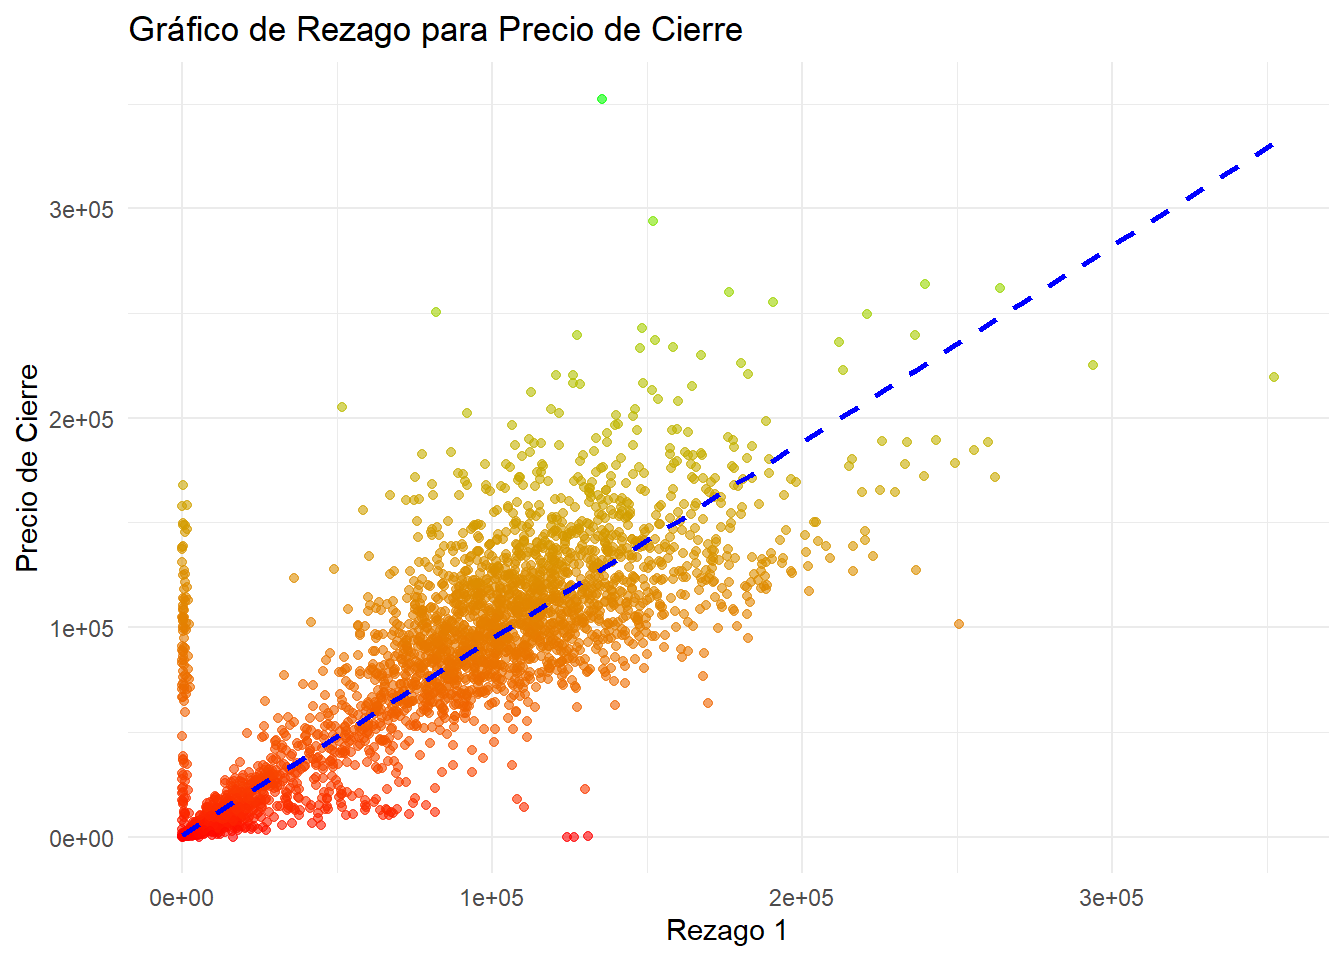
\includegraphics{bookdown-demo_files/figure-latex/unnamed-chunk-13-1.pdf}

Observaciones:

Entre los años 2013 y mediados del 2014 se puede ver cambios en la tendencia de la serie de tiempo de futuros de la soya, tamto para el promedio movil de 200 días, como para el de 500 días el cual es mas marcado.

Entre los años 2021 y mediados del 2023 se puede ver cambios en la tendencia de la serie de tiempo de futuros de la soya, tamto para el promedio movil de 200 días, como para el de 500 días el cual es mas marcado.Se podria llegar a validar por medio de un mayor estudio de este tiempo si la afectación fue causada por el desarrollo de la pandemia del covid-19 la cul inicio en marzo de 2020 e inicio a retrocer en Agosto de 2021 cuando se inicio el uso de las vacunas.

Al suavizar las fluctuaciones menores, a traves de los promedios móviles se logro resaltar las tendencias subyacentes en los datos.

\hypertarget{rezago}{%
\chapter{Rezago}\label{rezago}}

El concepto de rezago es fundamental para analizar y modelar series de tiempo porque permite entender cómo los valores pasados pueden influir en los valores presentes o futuros de la serie. Al analizar los rezagos, podemos identificar patrones, hacer predicciones más precisas y entender mejor la dinámica subyacente de los datos.

\begin{Shaded}
\begin{Highlighting}[]
\CommentTok{\# Sin cargar la librería dplyr para evitar conflictos}
\NormalTok{datos\_lag }\OtherTok{\textless{}{-}} \FunctionTok{data.frame}\NormalTok{(}
  \AttributeTok{Close =} \FunctionTok{as.numeric}\NormalTok{(}\FunctionTok{coredata}\NormalTok{(soybean\_xts)),}
  \AttributeTok{Lag =} \FunctionTok{as.numeric}\NormalTok{(}\FunctionTok{coredata}\NormalTok{(stats}\SpecialCharTok{::}\FunctionTok{lag}\NormalTok{(soybean\_xts))) }\CommentTok{\# Usar }
  \CommentTok{\# stats::lag para evitar conflictos}
\NormalTok{)}

\CommentTok{\# Comprobando que ambos vectores tengan la misma longitud}
\FunctionTok{stopifnot}\NormalTok{(}\FunctionTok{length}\NormalTok{(datos\_lag}\SpecialCharTok{$}\NormalTok{Close) }\SpecialCharTok{==} \FunctionTok{length}\NormalTok{(datos\_lag}\SpecialCharTok{$}\NormalTok{Lag))  }
\CommentTok{\# Detiene la ejecución si no son TRUE}

\CommentTok{\# Crear el gráfico de rezago con ggplot2}
\FunctionTok{library}\NormalTok{(ggplot2)}
\FunctionTok{ggplot}\NormalTok{(datos\_lag, }\FunctionTok{aes}\NormalTok{(}\AttributeTok{x=}\NormalTok{Lag, }\AttributeTok{y=}\NormalTok{Close)) }\SpecialCharTok{+}
  \FunctionTok{geom\_point}\NormalTok{(}\FunctionTok{aes}\NormalTok{(}\AttributeTok{color =}\NormalTok{ Close), }\AttributeTok{alpha=}\FloatTok{0.6}\NormalTok{) }\SpecialCharTok{+}
  \FunctionTok{geom\_smooth}\NormalTok{(}\AttributeTok{method =} \StringTok{\textquotesingle{}lm\textquotesingle{}}\NormalTok{, }\AttributeTok{se =} \ConstantTok{FALSE}\NormalTok{, }\AttributeTok{color=}\StringTok{"blue"}\NormalTok{, }
  \AttributeTok{linetype=}\StringTok{"dashed"}\NormalTok{) }\SpecialCharTok{+}
  \FunctionTok{scale\_color\_gradient}\NormalTok{(}\AttributeTok{low=}\StringTok{"red"}\NormalTok{, }\AttributeTok{high=}\StringTok{"green"}\NormalTok{) }\SpecialCharTok{+}
  \FunctionTok{theme\_minimal}\NormalTok{() }\SpecialCharTok{+}
  \FunctionTok{labs}\NormalTok{(}\AttributeTok{title=}\StringTok{"Gráfico de Rezago para Precio de Cierre"}\NormalTok{, }
  \AttributeTok{x=}\StringTok{"Rezago 1"}\NormalTok{, }\AttributeTok{y=}\StringTok{"Precio de Cierre"}\NormalTok{) }\SpecialCharTok{+}
  \FunctionTok{theme}\NormalTok{(}\AttributeTok{legend.position=}\StringTok{"none"}\NormalTok{)}
\end{Highlighting}
\end{Shaded}

\begin{verbatim}
## `geom_smooth()` using formula = 'y ~ x'
\end{verbatim}

\begin{verbatim}
## Warning: Removed 5 rows containing non-finite values (`stat_smooth()`).
\end{verbatim}

\begin{verbatim}
## Warning: Removed 5 rows containing missing values (`geom_point()`).
\end{verbatim}

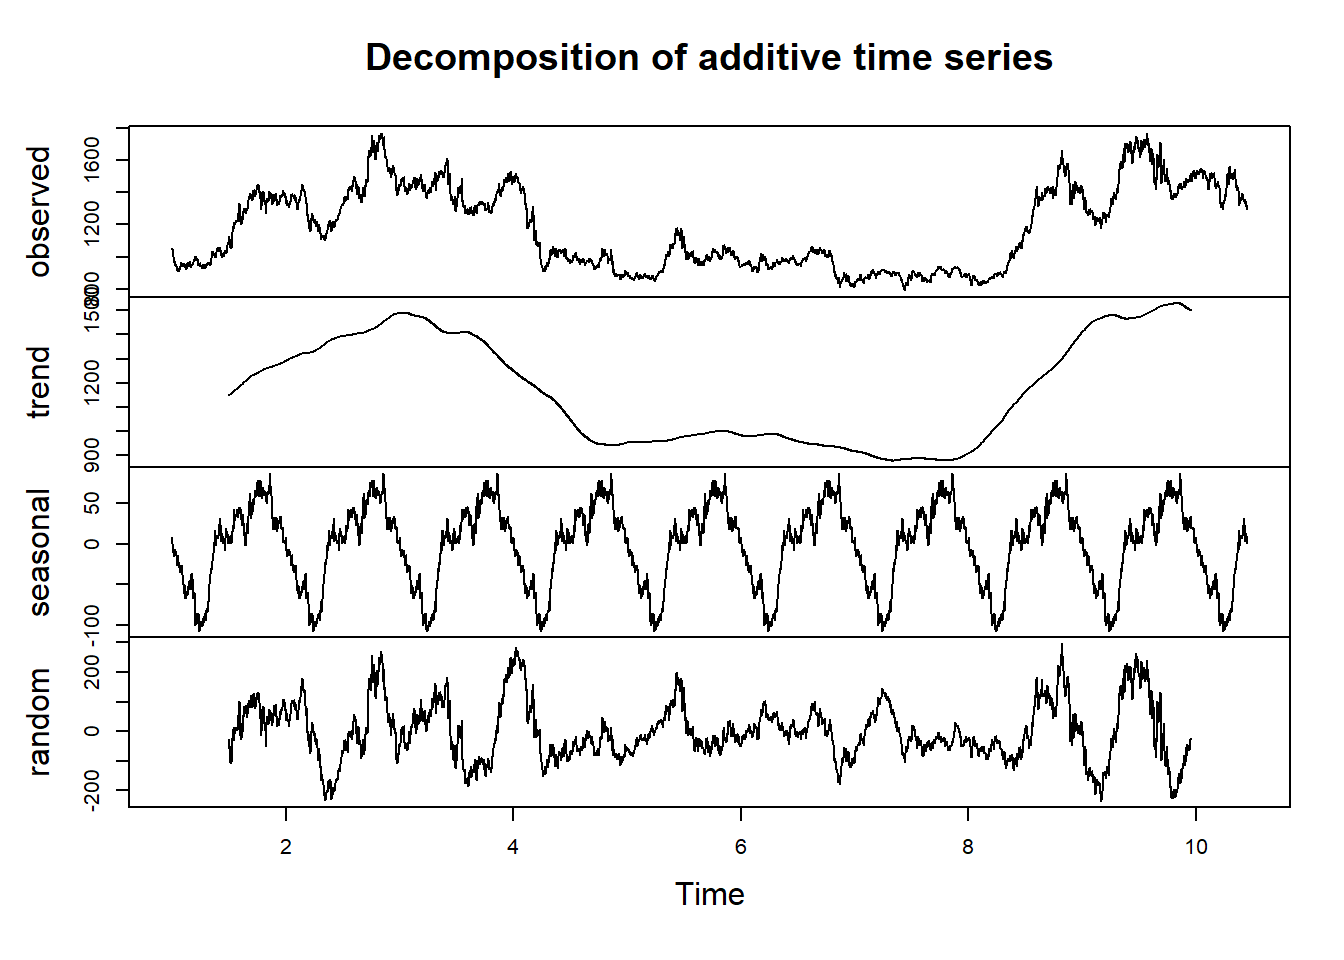
\includegraphics{bookdown-demo_files/figure-latex/unnamed-chunk-14-1.pdf}

\begin{Shaded}
\begin{Highlighting}[]
\CommentTok{\#library(forecast)}
\CommentTok{\#class(soybean\_xts) }
\CommentTok{\#as.ts(soybean\_xts)}
\CommentTok{\#modelo\textless{}{-}auto.arima(soybean\_xts)}
\CommentTok{\#modelo}

 \CommentTok{\#soybean\_tsp \textless{}{-} diff(soybean\_xts)}
\CommentTok{\#print(soybean\_tsp)}
\end{Highlighting}
\end{Shaded}

Se ve un patrón claro o una agrupación de puntos en el gráfico de rezago 1, por lo tanto es probable que exista una autocorrelación significativa. Se puede considerar modelos de series de tiempo como ARIMA que toman en cuenta la autocorrelación para hacer predicciones más precisas de ser necesario.

\hypertarget{descomposicion}{%
\chapter{Descomposicion}\label{descomposicion}}

Se refiere a los patrones o tendencias que se repiten a intervalos regulares, como cada día, mes, trimestre o año, dependiendo de la frecuencia de los datos. En otras palabras, es como un ciclo que se repite en el tiempo.

DESCOMPOSICION

Con la funcion decompose podemos hallar la:

Observed: Serie de tiempo original.

Tendencia (trend): Muestra la dirección general en la que se mueven los datos a largo plazo, sin tener en cuenta las fluctuaciones estacionales o irregulares.

Estacionalidad (seasonal): Representa las fluctuaciones que ocurren en intervalos regulares, como los cambios diarios, mensuales o anuales, debido a la estacionalidad.

Error o Residuo (random): Es la parte de la serie de tiempo que no se puede atribuir ni a la tendencia ni a la estacionalidad. Captura la variabilidad en los datos que no se puede explicar por los otros dos componentes.

\begin{Shaded}
\begin{Highlighting}[]
\CommentTok{\# Convertir a objeto ts, aquí supondré que tienes datos diarios.}
\NormalTok{frecuencia }\OtherTok{\textless{}{-}} \DecValTok{365}  \CommentTok{\# (12 para mensual, 4 para trimestral, etc.)}
\NormalTok{soybean\_ts }\OtherTok{\textless{}{-}} \FunctionTok{ts}\NormalTok{(soybean\_xts[, }\StringTok{"ZS.F.Close"}\NormalTok{], }
\AttributeTok{frequency =}\NormalTok{ frecuencia)}

\CommentTok{\# Utilizar decompose}
\NormalTok{soybean\_decomposed }\OtherTok{\textless{}{-}} \FunctionTok{decompose}\NormalTok{(soybean\_ts)}
\FunctionTok{plot}\NormalTok{(soybean\_decomposed)}
\end{Highlighting}
\end{Shaded}

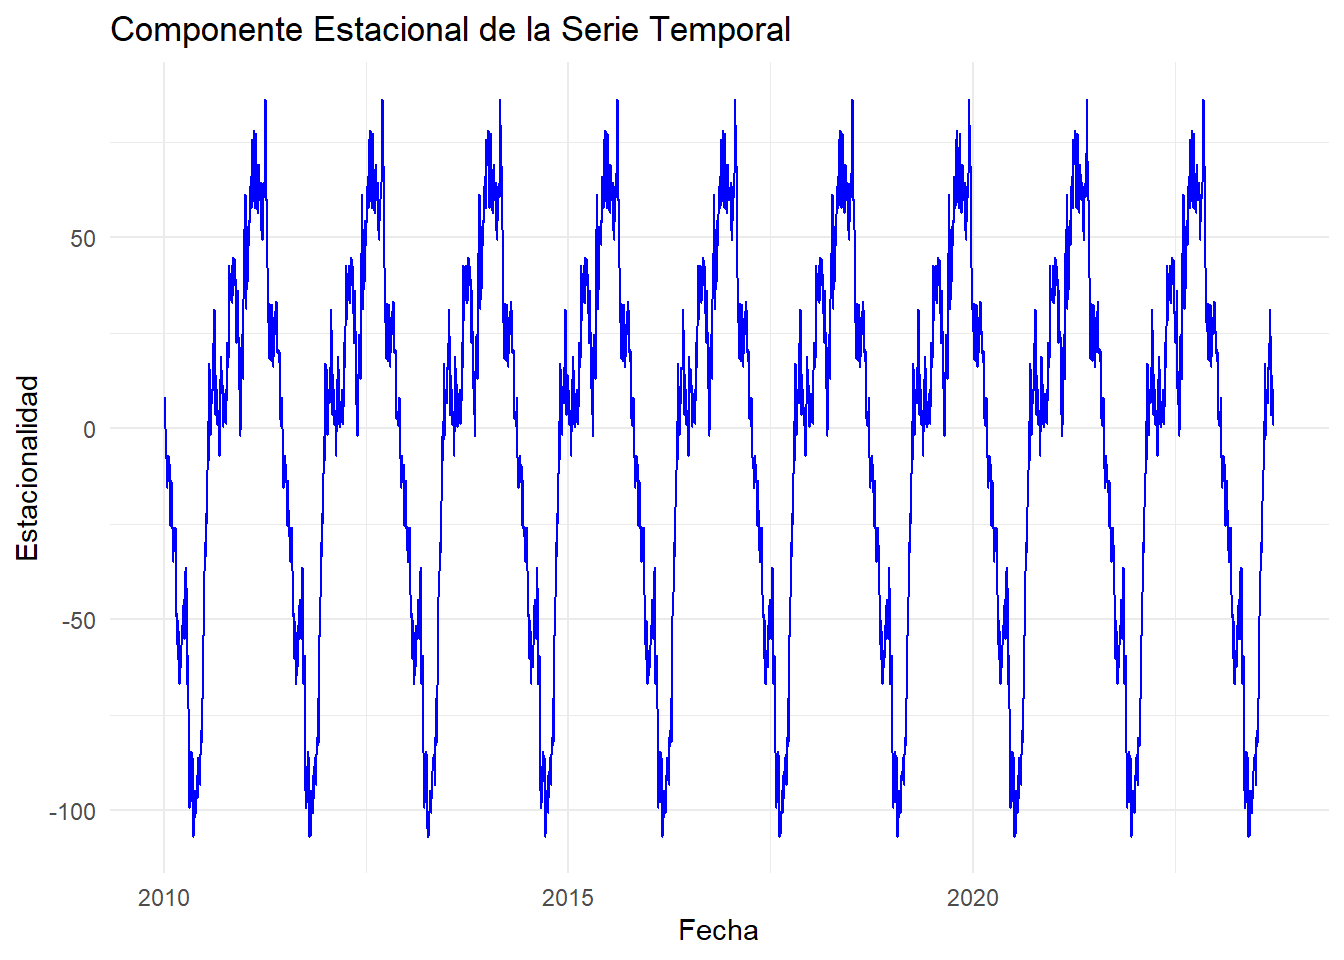
\includegraphics{bookdown-demo_files/figure-latex/unnamed-chunk-16-1.pdf}
Al validar el componenete estacional de la serie por separado, como se ve en la siguiente imagen:

\begin{Shaded}
\begin{Highlighting}[]
\CommentTok{\# Extraer el componente estacional y convertir el tiempo en fecha}
\NormalTok{seasonal\_df }\OtherTok{\textless{}{-}} \FunctionTok{data.frame}\NormalTok{(}
  \AttributeTok{Date =} \FunctionTok{as.Date}\NormalTok{(}\FunctionTok{index}\NormalTok{(soybean\_xts)),}
  \AttributeTok{Seasonal =} \FunctionTok{as.numeric}\NormalTok{(soybean\_decomposed}\SpecialCharTok{$}\NormalTok{seasonal)}
\NormalTok{)}

\CommentTok{\# Eliminar las filas con NA en el componente estacional (pueden }
\CommentTok{\# aparecer dependiendo del método de descomposición)}
\NormalTok{seasonal\_df }\OtherTok{\textless{}{-}}\NormalTok{ seasonal\_df[}\SpecialCharTok{!}\FunctionTok{is.na}\NormalTok{(seasonal\_df}\SpecialCharTok{$}\NormalTok{Seasonal), ]}
\end{Highlighting}
\end{Shaded}

\begin{Shaded}
\begin{Highlighting}[]
\FunctionTok{library}\NormalTok{(ggplot2)}

\FunctionTok{ggplot}\NormalTok{(seasonal\_df, }\FunctionTok{aes}\NormalTok{(}\AttributeTok{x=}\NormalTok{Date, }\AttributeTok{y=}\NormalTok{Seasonal)) }\SpecialCharTok{+}
  \FunctionTok{geom\_line}\NormalTok{(}\AttributeTok{color=}\StringTok{"blue"}\NormalTok{) }\SpecialCharTok{+}
  \FunctionTok{theme\_minimal}\NormalTok{() }\SpecialCharTok{+}
  \FunctionTok{labs}\NormalTok{(}\AttributeTok{title=}\StringTok{"Componente Estacional de la Serie Temporal"}\NormalTok{, }\AttributeTok{x=}\StringTok{"Fecha"}\NormalTok{, }\AttributeTok{y=}\StringTok{"Estacionalidad"}\NormalTok{) }\SpecialCharTok{+}
  \FunctionTok{theme}\NormalTok{(}\AttributeTok{legend.position=}\StringTok{"none"}\NormalTok{)}
\end{Highlighting}
\end{Shaded}

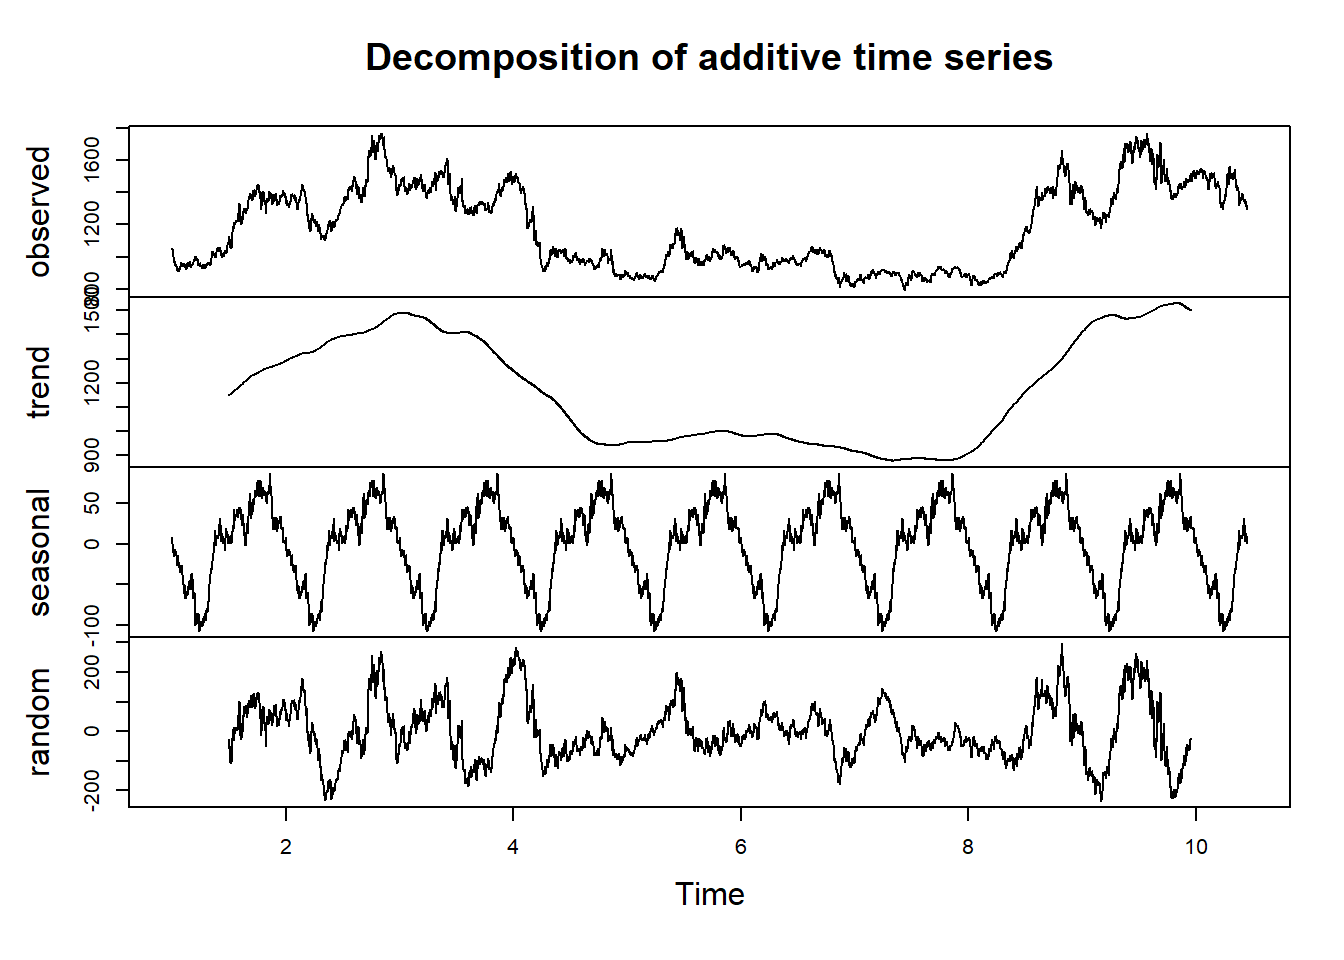
\includegraphics{bookdown-demo_files/figure-latex/unnamed-chunk-18-1.pdf}
Podemos deducir que la serie de tiempo de los precios del aceite de soya:

\begin{enumerate}
\def\labelenumi{\arabic{enumi}.}
\item
  Muestra patrones claros y consistentes, esto sugiere que la serie temporal tiene ciclos regulares que se repiten a intervalos fijos.
\item
  Se pueden identificar en qué momentos del ciclo tienden a ocurrir los valores altos y bajos de la serie.
\end{enumerate}

\hypertarget{estacionariedad}{%
\chapter{Estacionariedad}\label{estacionariedad}}

La prueba de Dickey-Fuller, específicamente el test ADF (Augmented Dickey-Fuller), es una prueba estadística utilizada para determinar si una serie temporal tiene una raíz unitaria, es decir, si es no estacionaria y presenta alguna forma de estructura temporal como una tendencia o una estacionalidad.

Vamos a comprobar mediante esta prueba si es o no estacionaria la serie de tiempo del precio del aceite de soya.

\begin{Shaded}
\begin{Highlighting}[]
\CommentTok{\# Cargar el paquete necesario}
\FunctionTok{library}\NormalTok{(tseries)}
\end{Highlighting}
\end{Shaded}

\begin{verbatim}
## Warning: package 'tseries' was built under R version 4.2.3
\end{verbatim}

\begin{Shaded}
\begin{Highlighting}[]
\CommentTok{\# Supón que tienes una serie temporal llamada \textquotesingle{}mi\_serie\textquotesingle{}}
\CommentTok{\# Realizar la prueba de Dickey{-}Fuller Aumentada}
\NormalTok{resultado\_adf }\OtherTok{\textless{}{-}} \FunctionTok{adf.test}\NormalTok{(soybean\_ts)}

\CommentTok{\# Imprimir el resultado}
\FunctionTok{print}\NormalTok{(resultado\_adf)}
\end{Highlighting}
\end{Shaded}

\begin{verbatim}
## 
##  Augmented Dickey-Fuller Test
## 
## data:  soybean_ts
## Dickey-Fuller = -2.0408, Lag order = 15, p-value = 0.5611
## alternative hypothesis: stationary
\end{verbatim}

Cuando hacemos una prueba como esta, estamos tratando de averiguar si la serie de tiempo es ``estacionaria'' o no. Una serie estacionaria es aquella cuyas propiedades, como la media y la varianza, no cambian con el tiempo.

En esta prueba, tenemos algo llamado valor p, que es como un termómetro que nos dice qué tan seguros estamos de si la serie de tiempo es estacionaria o no. Un valor p pequeño (menor que 0.05) nos dice: ``La serie es estacionaria''. Un valor p grande (mayor que 0.05) nos dice: ``La serie no es estacionaria''.

En este caso, el valor p es 0.5657, que es bastante grande, así que, la serie de tiempo no es estacionaria.

\hypertarget{diferenciacion}{%
\chapter{Diferenciacion}\label{diferenciacion}}

Diferenciar una serie temporal es un proceso utilizado para hacer que una serie no estacionaria se vuelva estacionaria. La idea es transformar la serie de datos para estabilizar la media de la serie temporal, eliminando tendencias y efectos estacionales. En otras palabras, se busca que las propiedades de la serie (como la media y la varianza) no cambien con el tiempo.

\begin{Shaded}
\begin{Highlighting}[]
\CommentTok{\# Inicializa un contador para las diferenciaciones}
\NormalTok{diferencias }\OtherTok{\textless{}{-}} \DecValTok{0}

\CommentTok{\# Realiza el test ADF y verifica la estacionariedad}
\ControlFlowTok{while}\NormalTok{(}\ConstantTok{TRUE}\NormalTok{) \{}
\NormalTok{  p\_value }\OtherTok{\textless{}{-}} \FunctionTok{adf.test}\NormalTok{(soybean\_ts)}\SpecialCharTok{$}\NormalTok{p.value}
  \FunctionTok{cat}\NormalTok{(}\StringTok{"Número de diferencias:"}\NormalTok{, diferencias, }\StringTok{"{-} Valor p:"}\NormalTok{, }
\NormalTok{  p\_value, }\StringTok{"}\SpecialCharTok{\textbackslash{}n}\StringTok{"}\NormalTok{)}
  
  \CommentTok{\# Si el valor p es menor que 0.05, la serie es estacionaria,}
  \CommentTok{\# y puedes salir del bucle.}
  \ControlFlowTok{if}\NormalTok{(p\_value }\SpecialCharTok{\textless{}} \FloatTok{0.05}\NormalTok{) \{}
    \FunctionTok{cat}\NormalTok{(}\StringTok{"La serie se volvió estacionaria después de"}\NormalTok{, diferencias, }\StringTok{"diferenciaciones.}\SpecialCharTok{\textbackslash{}n}\StringTok{"}\NormalTok{)}
    \ControlFlowTok{break}
\NormalTok{  \}}
  
  \CommentTok{\# Si has llegado al final de la serie, sal del bucle}
  \ControlFlowTok{if}\NormalTok{(}\FunctionTok{length}\NormalTok{(soybean\_ts) }\SpecialCharTok{\textless{}=} \DecValTok{1}\NormalTok{) \{}
    \FunctionTok{cat}\NormalTok{(}\StringTok{"La serie no se volvió estacionaria después de }
\StringTok{        diferenciar.}\SpecialCharTok{\textbackslash{}n}\StringTok{"}\NormalTok{)}
    \ControlFlowTok{break}
\NormalTok{  \}}
  
  \CommentTok{\# Si no es estacionaria, diferenciar la serie una vez más y }
  \CommentTok{\# continuar el bucle.}
\NormalTok{  soybean\_ts }\OtherTok{\textless{}{-}} \FunctionTok{diff}\NormalTok{(soybean\_ts)}
\NormalTok{  diferencias }\OtherTok{\textless{}{-}}\NormalTok{ diferencias }\SpecialCharTok{+} \DecValTok{1}
\NormalTok{\}}
\end{Highlighting}
\end{Shaded}

\begin{verbatim}
## Número de diferencias: 0 - Valor p: 0.5610549
\end{verbatim}

\begin{verbatim}
## Warning in adf.test(soybean_ts): p-value smaller than printed p-value
\end{verbatim}

\begin{verbatim}
## Número de diferencias: 1 - Valor p: 0.01 
## La serie se volvió estacionaria después de 1 diferenciaciones.
\end{verbatim}

Conclusión:

Antes de realizar cualquier diferenciación (d = 0), el valor p de la prueba de Dickey-Fuller Aumentada es 0.5657422, lo que es mayor que 0.05. Por lo tanto, no puedes rechazar la hipótesis nula de que existe una raíz unitaria, y se concluye que la serie original no es estacionaria.

Después de diferenciar la serie una vez (d = 1), el valor p de la prueba de Dickey-Fuller Aumentada es 0.01, lo cual es menor que 0.05.

La serie de tiempo original no es estacionaria, pero después de realizar una diferenciación, la serie resultante sí es estacionaria.

Fue necesario transformarla o diferenciarla para eliminar la tendencia y estabilizar la varianza, antes de aplicar modelos de series temporales como ARIMA.

\hypertarget{holter-winter}{%
\chapter{Holter-Winter}\label{holter-winter}}

La metodología Holt-Winters, también conocida como triple suavizado exponencial, es útil para series de tiempo con componentes de tendencia y estacionalidad.

\begin{Shaded}
\begin{Highlighting}[]
\FunctionTok{library}\NormalTok{(forecast)  }\CommentTok{\# Necesario para pronosticar con el modelo }
\end{Highlighting}
\end{Shaded}

\begin{verbatim}
## Warning: package 'forecast' was built under R version 4.2.3
\end{verbatim}

\begin{Shaded}
\begin{Highlighting}[]
\CommentTok{\# Holt{-}Winters}



\CommentTok{\# Ajustar el modelo Holt{-}Winters}
\NormalTok{hw\_model }\OtherTok{\textless{}{-}} \FunctionTok{HoltWinters}\NormalTok{(soybean\_ts)}
\CommentTok{\# Visualizar componentes del modelo}
\FunctionTok{plot}\NormalTok{(hw\_model)}
\end{Highlighting}
\end{Shaded}

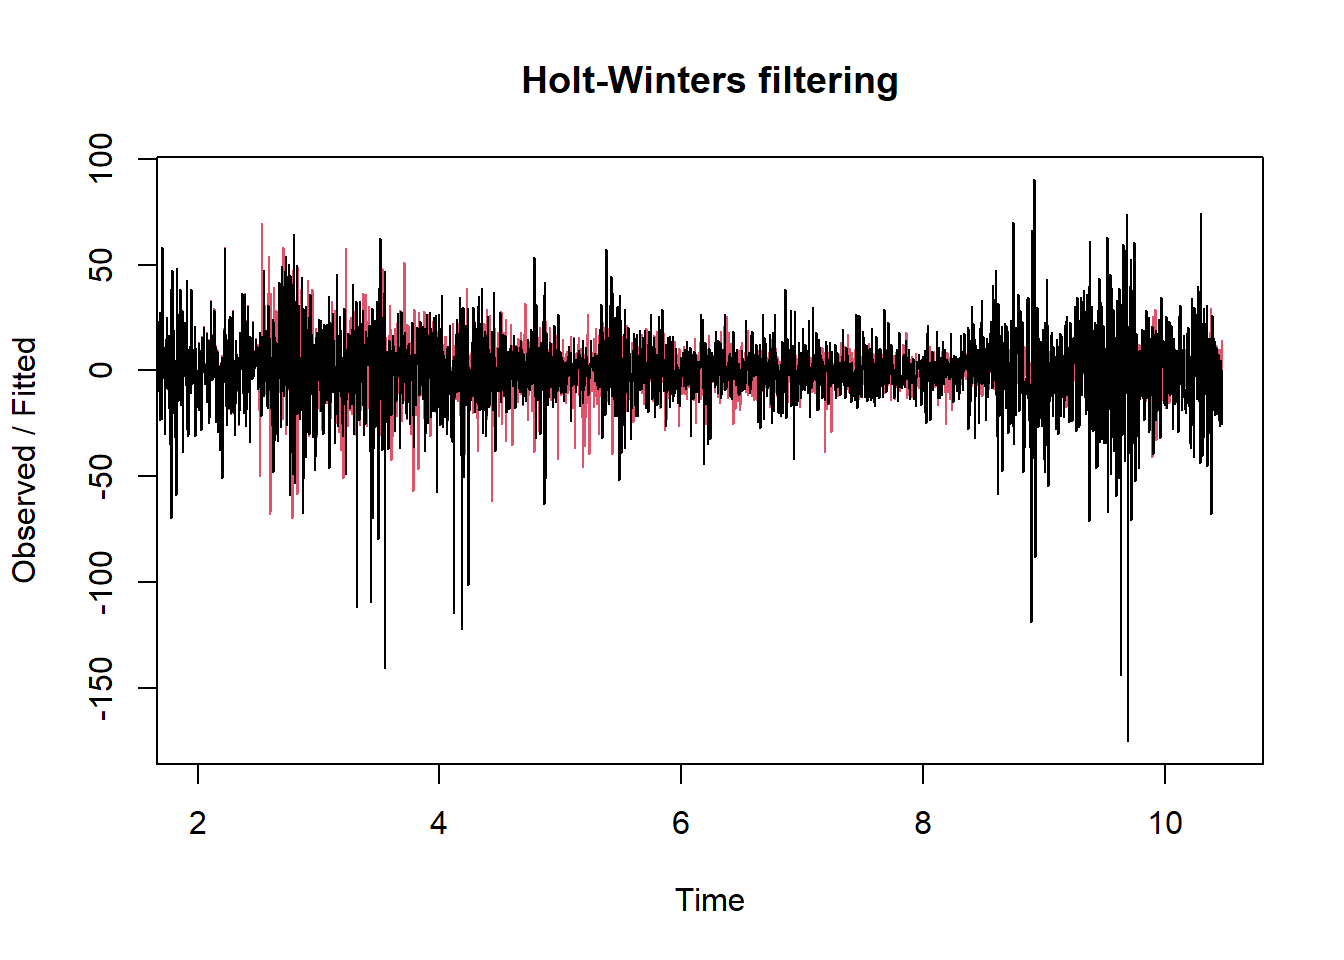
\includegraphics{bookdown-demo_files/figure-latex/unnamed-chunk-21-1.pdf}

\begin{Shaded}
\begin{Highlighting}[]
\CommentTok{\# Pronosticar los siguientes 30 días (o la cantidad que desees)}
\FunctionTok{library}\NormalTok{(forecast)}
\NormalTok{hw\_forecast }\OtherTok{\textless{}{-}} \FunctionTok{forecast}\NormalTok{(hw\_model, }\AttributeTok{h =} \DecValTok{30}\NormalTok{)  }\CommentTok{\# Cambia 30 por el }
\CommentTok{\# número de periodos que quieras pronosticar}
\FunctionTok{plot}\NormalTok{(hw\_forecast)}
\end{Highlighting}
\end{Shaded}

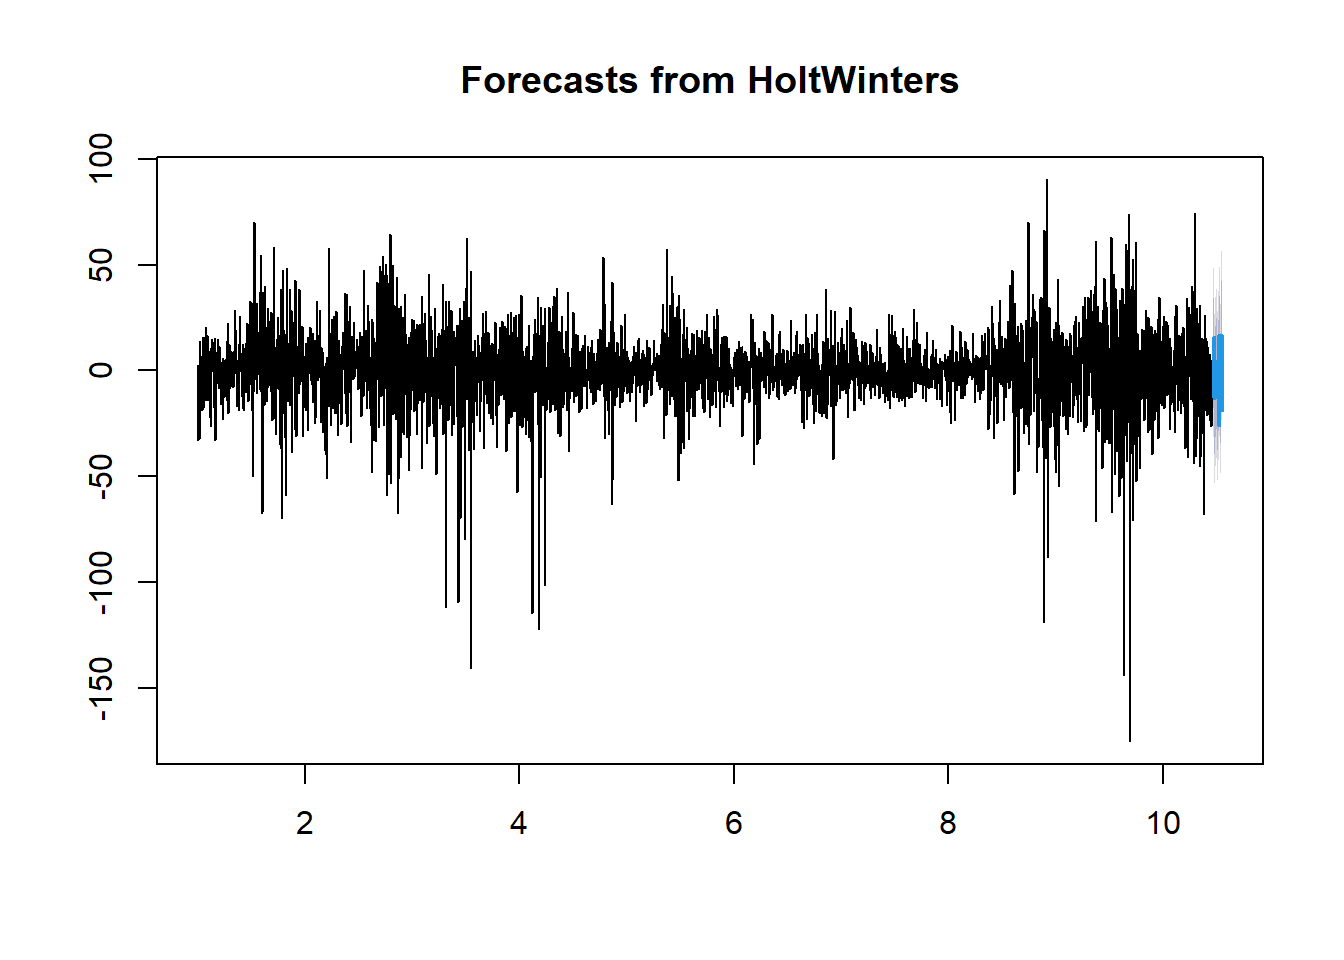
\includegraphics{bookdown-demo_files/figure-latex/unnamed-chunk-22-1.pdf}

\begin{Shaded}
\begin{Highlighting}[]
\CommentTok{\# Revisar detalles del modelo y del pronóstico}
\FunctionTok{summary}\NormalTok{(hw\_model)}
\end{Highlighting}
\end{Shaded}

\begin{verbatim}
##              Length Class  Mode     
## fitted       12364  mts    numeric  
## x             3456  ts     numeric  
## alpha            1  -none- numeric  
## beta             1  -none- numeric  
## gamma            1  -none- numeric  
## coefficients   367  -none- numeric  
## seasonal         1  -none- character
## SSE              1  -none- numeric  
## call             2  -none- call
\end{verbatim}

\begin{Shaded}
\begin{Highlighting}[]
\FunctionTok{summary}\NormalTok{(hw\_forecast)}
\end{Highlighting}
\end{Shaded}

\begin{verbatim}
## 
## Forecast method: HoltWinters
## 
## Model Information:
## Holt-Winters exponential smoothing with trend and additive seasonal component.
## 
## Call:
## HoltWinters(x = soybean_ts)
## 
## Smoothing parameters:
##  alpha: 0.001521614
##  beta : 0
##  gamma: 0.3511517
## 
## Coefficients:
##               [,1]
## a     -1.984582580
## b     -0.001484417
## s1    10.314656534
## s2    17.874294874
## s3     5.232474330
## s4   -11.293771948
## s5     0.951602577
## s6     3.006374310
## s7     1.759498869
## s8    -3.341989784
## s9    -0.314377212
## s10   -6.228944388
## s11    0.497178737
## s12    6.215103894
## s13    4.783045092
## s14   -4.138468694
## s15   -9.664046098
## s16    3.719584563
## s17    6.861089813
## s18   -0.336699222
## s19   18.716821596
## s20  -23.742818413
## s21   11.526675054
## s22   -6.086538594
## s23   11.342669819
## s24    6.815182886
## s25   -6.402688781
## s26    1.177083882
## s27    0.679908084
## s28   18.795027718
## s29   10.316408539
## s30  -16.705414792
## s31    7.121920397
## s32   18.938106635
## s33   -4.208132861
## s34    2.577424683
## s35   10.692427210
## s36    5.328611242
## s37    8.663030408
## s38    3.637183387
## s39  -10.880338048
## s40   -1.976077764
## s41    0.958449900
## s42   10.187700338
## s43    4.132360622
## s44   -5.166570831
## s45   -6.594768964
## s46  -21.103794596
## s47   12.897839890
## s48    7.713430395
## s49   16.681211531
## s50   -0.179922901
## s51   -4.682626689
## s52  -18.521924918
## s53  -14.075674049
## s54  -12.690886521
## s55   15.034759913
## s56   16.963630423
## s57    7.270399771
## s58  -20.720350585
## s59    1.995831506
## s60    6.091075530
## s61  -52.134254821
## s62   14.356251661
## s63   -8.409259122
## s64   -9.235965403
## s65   -6.007951361
## s66   11.029091204
## s67    2.800534223
## s68   27.430891931
## s69   18.008679655
## s70   14.666383557
## s71    8.668020638
## s72  -16.152771549
## s73   -8.297463525
## s74   -1.280376526
## s75   30.468180599
## s76   10.209686452
## s77   -0.137761283
## s78   26.060326969
## s79   -1.423837395
## s80   12.778035533
## s81  -13.396812030
## s82  -60.591451302
## s83   -6.613355861
## s84   11.389141648
## s85    7.644408211
## s86   -9.985301091
## s87   14.053193852
## s88   19.186089335
## s89    0.535677198
## s90   -2.875700559
## s91   17.712287231
## s92  -28.123393878
## s93    0.798539011
## s94   -0.496192644
## s95   -5.823785474
## s96   12.681696916
## s97   -5.306739950
## s98  -10.653774888
## s99    0.411304410
## s100   0.416542312
## s101  38.535557692
## s102 -10.518202529
## s103  -7.738458083
## s104 -14.327093859
## s105  -2.768356823
## s106   9.075766064
## s107   2.461798818
## s108 -13.369906617
## s109   1.293348021
## s110  -5.512646557
## s111   0.150564813
## s112   7.032292593
## s113   6.313711157
## s114   4.225309798
## s115 -10.781181936
## s116  13.047966696
## s117   2.297076714
## s118   1.608034284
## s119  -7.771285399
## s120   4.547286094
## s121   0.895804140
## s122  10.282128411
## s123   1.807643948
## s124   3.073914110
## s125  -3.662082457
## s126   5.151901030
## s127  -1.522671168
## s128  -0.974093859
## s129   8.471023061
## s130   6.869424629
## s131 -20.895370096
## s132   1.533865851
## s133  -3.482646294
## s134   2.805026043
## s135  -5.994517284
## s136   8.938061573
## s137  11.032646671
## s138   3.108892126
## s139  -7.239974368
## s140   8.561669632
## s141   5.510033831
## s142   3.804039222
## s143  16.754341483
## s144  -9.336733335
## s145   2.726791639
## s146   3.399507135
## s147  -1.083861079
## s148  -5.551368048
## s149  -6.435410505
## s150  -2.011328528
## s151  -2.511906967
## s152  -9.718225120
## s153   1.827246273
## s154  -3.985772601
## s155 -17.624729314
## s156  18.911356075
## s157   9.965937088
## s158 -17.351889864
## s159   2.577317372
## s160  -1.238158494
## s161  -5.736239045
## s162  14.024105451
## s163   6.055250473
## s164  19.147428598
## s165  -8.529492467
## s166   8.076388126
## s167 -19.051167773
## s168   0.237971944
## s169   3.974754432
## s170  -2.580633551
## s171  13.153541183
## s172   3.116689962
## s173   1.119603690
## s174   0.323613312
## s175   4.952843723
## s176   3.254640033
## s177   3.567339958
## s178   4.011108373
## s179 -16.089402611
## s180  -7.694479724
## s181   0.774035356
## s182  14.999392882
## s183   5.606916879
## s184   2.986985325
## s185  -1.534739829
## s186   6.923109944
## s187  -4.672236823
## s188   2.951194744
## s189  -5.430172039
## s190   1.830893888
## s191  -0.450111374
## s192  -1.733976770
## s193  -6.956546994
## s194   4.678280726
## s195  15.626423849
## s196 -15.188449724
## s197   6.004818926
## s198  -2.663911124
## s199 -11.290916178
## s200  -1.724956745
## s201  -0.131381855
## s202   5.287530549
## s203  -1.728364295
## s204   8.451643027
## s205  -1.814096924
## s206  -0.491648590
## s207   3.594530883
## s208  -2.528860600
## s209  -3.393446638
## s210   1.004671786
## s211  -3.046892446
## s212  11.341802335
## s213  -1.534847490
## s214   2.495705435
## s215  -5.762434533
## s216  -4.768098478
## s217  -5.826680125
## s218   5.860029127
## s219   3.317051148
## s220  -0.134695032
## s221   9.107620755
## s222  -2.744692254
## s223  -1.405140716
## s224  -2.247577422
## s225  -0.736460251
## s226  -3.794069160
## s227   1.566676934
## s228  -9.758273599
## s229  -1.428994687
## s230  -7.977810765
## s231   6.628399817
## s232  -9.000719276
## s233  -5.452317047
## s234  -7.716233572
## s235   4.686069396
## s236   0.305629595
## s237   8.302369499
## s238   3.227602434
## s239   1.531554964
## s240  14.469930659
## s241  10.087736967
## s242   2.869987024
## s243  -5.054995298
## s244  -7.208881708
## s245   2.886803587
## s246   6.430753349
## s247   6.017576733
## s248  -1.276738887
## s249   1.200158057
## s250   8.006406746
## s251   2.382911353
## s252  -3.230114280
## s253  -6.244755815
## s254  -7.035181728
## s255 -10.345546115
## s256   0.756044440
## s257   2.317891166
## s258   0.591359849
## s259  12.972344243
## s260   7.470249420
## s261 -12.807911531
## s262   9.909897603
## s263  -2.181574126
## s264   9.061506322
## s265   4.602534041
## s266  -2.900748330
## s267  -8.625275116
## s268  -0.693312777
## s269  -6.406209817
## s270 -16.476443228
## s271  -7.868183819
## s272  -5.225796883
## s273   4.136882863
## s274 -13.030882038
## s275  11.815003474
## s276  -1.605732717
## s277   5.523779356
## s278   4.355798636
## s279  -0.142331930
## s280  -8.487392667
## s281  -2.423134311
## s282  14.777208007
## s283  10.975350048
## s284  -0.031725524
## s285   3.952668307
## s286   9.523439658
## s287   3.812772446
## s288  17.695794793
## s289  -4.092724679
## s290  10.372696211
## s291 -10.422300385
## s292  15.484932728
## s293  18.747098342
## s294  13.585975544
## s295  14.040247838
## s296  -6.211912171
## s297   4.083608818
## s298   5.109930488
## s299  -6.188641449
## s300 -10.957180738
## s301   5.345063701
## s302  25.587388423
## s303   0.714525431
## s304   2.414187190
## s305   2.127723347
## s306 -15.232323243
## s307   7.715676510
## s308   8.687302707
## s309  -2.925391283
## s310  13.048640996
## s311  -0.063179797
## s312   0.909600114
## s313  13.512916245
## s314   4.007937286
## s315   2.850754916
## s316   9.365804315
## s317  15.525244777
## s318  -1.249872728
## s319  20.683620623
## s320  -8.422959918
## s321 -12.851557824
## s322 -12.748313029
## s323  -2.427220804
## s324   2.468893178
## s325   3.649083115
## s326  10.910818659
## s327  -1.267107720
## s328  18.864402389
## s329   1.154519548
## s330 -24.338743221
## s331  10.692082763
## s332  17.173559209
## s333 -26.879175539
## s334   2.317715851
## s335  -1.803340177
## s336   8.669815203
## s337  10.774333618
## s338  -9.762994990
## s339   5.540778242
## s340   1.355306197
## s341   8.318763332
## s342  -1.121312910
## s343  -5.046428433
## s344   6.391044659
## s345  -4.579673607
## s346   6.225392239
## s347  -0.632907993
## s348  13.461125116
## s349 -12.926620058
## s350   5.759155294
## s351  -9.249725219
## s352  -8.050850342
## s353   6.218446988
## s354  -6.864900638
## s355  -6.868767973
## s356  -1.775186518
## s357   7.947714769
## s358   2.207334884
## s359  -0.962905330
## s360   9.327568653
## s361  -8.020286999
## s362   5.390884382
## s363   2.731310488
## s364  -2.120153614
## s365   2.381502063
## 
## Error measures:
##                     ME     RMSE      MAE MPE MAPE      MASE       ACF1
## Training set 0.3546955 20.36104 14.07105 NaN  Inf 0.7991731 0.02147927
## 
## Forecasts:
##          Point Forecast      Lo 80      Hi 80     Lo 95    Hi 95
## 10.47123      8.3285895 -17.765392 34.4225708 -31.57871 48.23589
## 10.47397     15.8867435 -10.207268 41.9807549 -24.02060 55.79409
## 10.47671      3.2434385 -22.850603 29.3374802 -36.66395 43.15083
## 10.47945    -13.2842922 -39.378364 12.8097797 -53.19173 26.62315
## 10.48219     -1.0404021 -27.134504 25.0537000 -40.94789 38.86708
## 10.48493      1.0128852 -25.081247 27.1070175 -38.89465 40.92042
## 10.48767     -0.2354746 -26.329637 25.8586879 -40.14305 39.67210
## 10.49041     -5.3384477 -31.432640 20.7557450 -45.24607 34.56918
## 10.49315     -2.3123195 -28.406542 23.7819034 -42.21999 37.59535
## 10.49589     -8.2283711 -34.322624 17.8658820 -48.13609 31.67935
## 10.49863     -1.5037324 -27.598016 24.5905509 -41.41149 38.40403
## 10.50137      4.2127083 -21.881605 30.3070218 -35.69510 44.12052
## 10.50411      2.7791651 -23.315179 28.8735088 -37.12869 42.68702
## 10.50685     -6.1438331 -32.238207 19.9505408 -46.05173 33.76407
## 10.50959    -11.6708949 -37.765299 14.4235092 -51.57884 28.23705
## 10.51233      1.7112513 -24.383183 27.8056857 -38.19674 41.61924
## 10.51507      4.8512722 -21.243192 30.9457367 -35.05677 44.75931
## 10.51781     -2.3480013 -28.442496 23.7464935 -42.25609 37.56008
## 10.52055     16.7040351  -9.390490 42.7985601 -23.20410 56.61217
## 10.52329    -25.7570893 -51.851645  0.3374659 -65.66527 14.15109
## 10.52603      9.5109197 -16.583666 35.6055051 -30.39730 49.41914
## 10.52877     -8.1037783 -34.198394 17.9908373 -48.01205 31.80449
## 10.53151      9.3239457 -16.770700 35.4185915 -30.58437 49.23226
## 10.53425      4.7949743 -21.299702 30.8896503 -35.11339 44.70334
## 10.53699     -8.4243818 -34.519088 17.6703244 -48.33279 31.48403
## 10.53973     -0.8460935 -26.940830 25.2486429 -40.75455 39.06236
## 10.54247     -1.3447537 -27.439520 24.7500129 -41.25326 38.56375
## 10.54521     16.7688815  -9.325915 42.8636783 -23.13967 56.67743
## 10.54795      8.2887779 -17.806049 34.3836049 -31.61982 48.19737
## 10.55068    -18.7345299 -44.829387  7.3603274 -58.64317 21.17411
\end{verbatim}

\hypertarget{arima}{%
\chapter{ARIMA}\label{arima}}

ARIMA es como un método o herramienta que nos ayuda a entender y prever cómo se comportará una secuencia de números en el futuro, basándose en cómo se ha comportado en el pasado.

\begin{Shaded}
\begin{Highlighting}[]
\NormalTok{modelo}\OtherTok{\textless{}{-}}\FunctionTok{auto.arima}\NormalTok{(soybean\_ts)}
\NormalTok{modelo}
\end{Highlighting}
\end{Shaded}

\begin{verbatim}
## Series: soybean_ts 
## ARIMA(0,0,0) with zero mean 
## 
## sigma^2 = 314.7:  log likelihood = -14842.62
## AIC=29687.25   AICc=29687.25   BIC=29693.39
\end{verbatim}

Conclusión:

El resultado de auto.arima() elige un modelo ARIMA(0,0,0) con media cero,indica según el análisis que no hay patrones, ritmos, ni tendencias claras en los datos de la serie de tiempo del precio del aceite de soya.

Los valores de la serie de tiempo del precio delaceite de soya son como un conjunto de números aleatorios, o ``ruido blanco'', sin conexión aparente entre ellos. En otras palabras, cada punto de datos es independiente de los otros y no está influenciado por los valores pasados en la serie.

\begin{Shaded}
\begin{Highlighting}[]
\FunctionTok{length}\NormalTok{(soybean\_ts)}
\end{Highlighting}
\end{Shaded}

\begin{verbatim}
## [1] 3456
\end{verbatim}

\begin{Shaded}
\begin{Highlighting}[]
\FunctionTok{sum}\NormalTok{(}\FunctionTok{is.na}\NormalTok{(soybean\_ts))}
\end{Highlighting}
\end{Shaded}

\begin{verbatim}
## [1] 0
\end{verbatim}

\begin{Shaded}
\begin{Highlighting}[]
\FunctionTok{class}\NormalTok{(soybean\_ts)}
\end{Highlighting}
\end{Shaded}

\begin{verbatim}
## [1] "ts"
\end{verbatim}

\begin{Shaded}
\begin{Highlighting}[]
\FunctionTok{sum}\NormalTok{(}\FunctionTok{is.na}\NormalTok{(soybean\_ts) }\SpecialCharTok{|} \FunctionTok{is.infinite}\NormalTok{(soybean\_ts))}
\end{Highlighting}
\end{Shaded}

\begin{verbatim}
## [1] 0
\end{verbatim}

\begin{Shaded}
\begin{Highlighting}[]
\CommentTok{\# Instalar el paquete changepoint}
\CommentTok{\#install.packages("changepoint")}

\CommentTok{\# Cargar el paquete changepoint}
\FunctionTok{library}\NormalTok{(changepoint)}
\end{Highlighting}
\end{Shaded}

\begin{verbatim}
## Warning: package 'changepoint' was built under R version 4.2.3
\end{verbatim}

\begin{verbatim}
## Successfully loaded changepoint package version 2.2.4
##  See NEWS for details of changes.
\end{verbatim}

\begin{Shaded}
\begin{Highlighting}[]
\NormalTok{mval\_soybean }\OtherTok{\textless{}{-}} \FunctionTok{cpt.mean}\NormalTok{(}\FunctionTok{as.numeric}\NormalTok{(soybean\_ts), }\AttributeTok{method =} \StringTok{"AMOC"}\NormalTok{)}
\FunctionTok{cpts}\NormalTok{(mval\_soybean)}
\end{Highlighting}
\end{Shaded}

\begin{verbatim}
## [1] 3410
\end{verbatim}

\begin{Shaded}
\begin{Highlighting}[]
\CommentTok{\# Plot de la serie de tiempo}
\FunctionTok{plot}\NormalTok{(soybean\_ts, }\AttributeTok{type=}\StringTok{\textquotesingle{}l\textquotesingle{}}\NormalTok{, }\AttributeTok{main=}\StringTok{\textquotesingle{}Serie de Tiempo con Punto de Cambio\textquotesingle{}}\NormalTok{, }\AttributeTok{ylab=}\StringTok{\textquotesingle{}Valor\textquotesingle{}}\NormalTok{, }\AttributeTok{xlab=}\StringTok{\textquotesingle{}Tiempo\textquotesingle{}}\NormalTok{)}

\CommentTok{\# Añadir una línea vertical en el punto de cambio}
\FunctionTok{abline}\NormalTok{(}\AttributeTok{v=}\DecValTok{3410}\NormalTok{, }\AttributeTok{col=}\StringTok{\textquotesingle{}red\textquotesingle{}}\NormalTok{, }\AttributeTok{lty=}\DecValTok{2}\NormalTok{, }\AttributeTok{lwd=}\DecValTok{2}\NormalTok{)}

\CommentTok{\# Añadir una leyenda}
\FunctionTok{legend}\NormalTok{(}\StringTok{"topright"}\NormalTok{, }\AttributeTok{legend=}\StringTok{"Punto de Cambio"}\NormalTok{, }\AttributeTok{col=}\StringTok{"red"}\NormalTok{, }\AttributeTok{lty=}\DecValTok{2}\NormalTok{, }\AttributeTok{lwd=}\DecValTok{2}\NormalTok{)}
\end{Highlighting}
\end{Shaded}

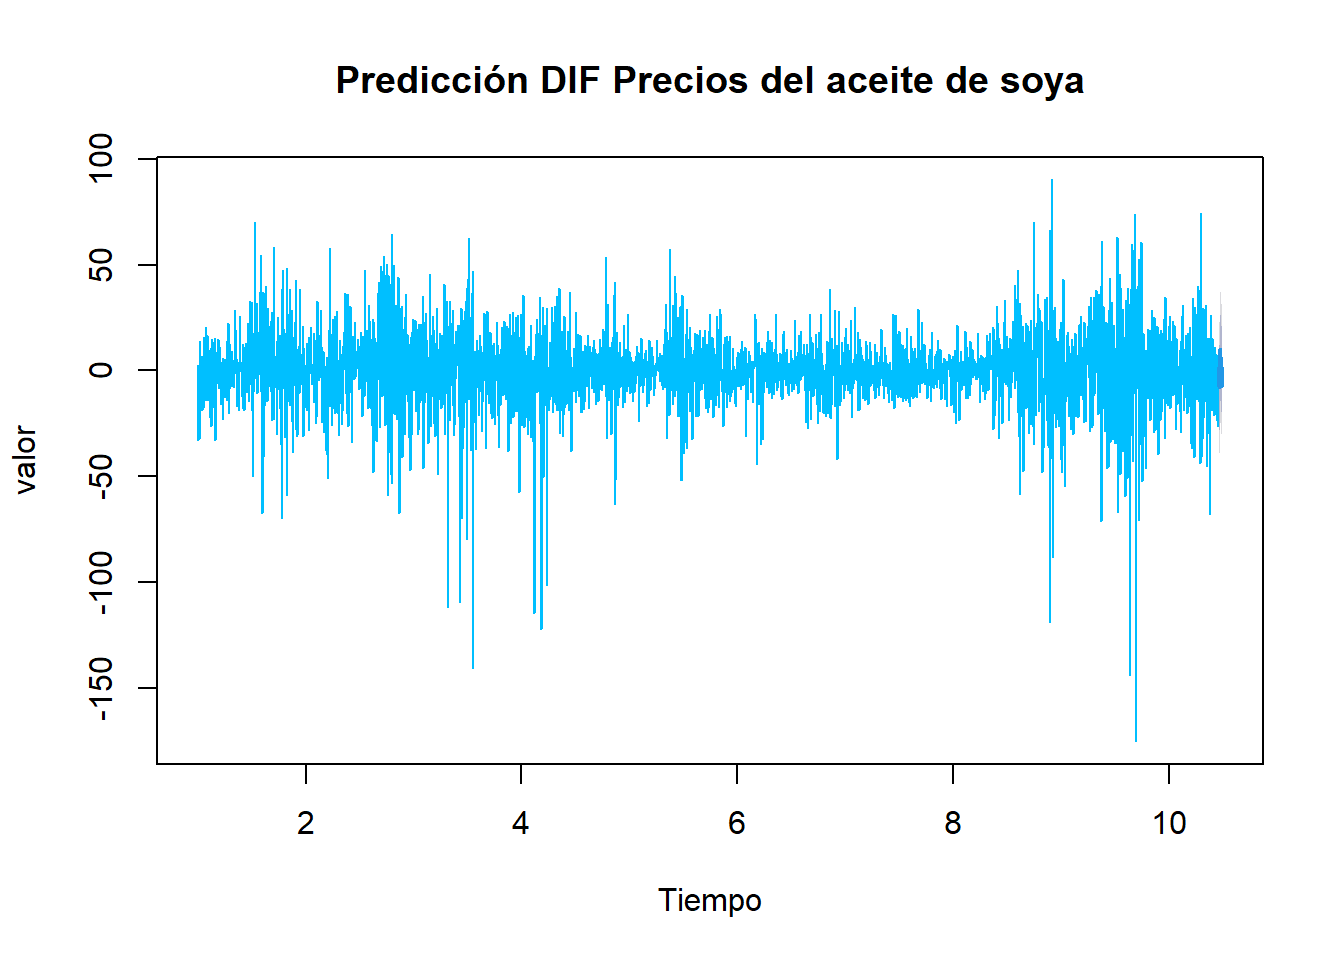
\includegraphics{bookdown-demo_files/figure-latex/unnamed-chunk-27-1.pdf}

\begin{Shaded}
\begin{Highlighting}[]
\NormalTok{pred}\OtherTok{\textless{}{-}}\FunctionTok{forecast}\NormalTok{(soybean\_ts,}\AttributeTok{h=}\DecValTok{12}\NormalTok{)}
\NormalTok{pred}
\end{Highlighting}
\end{Shaded}

\begin{verbatim}
##          Point Forecast     Lo 80    Hi 80     Lo 95    Hi 95
## 10.47123      9.1621457 -11.04269 29.36699 -21.73849 40.06278
## 10.47397      9.7073395 -10.49750 29.91218 -21.19330 40.60797
## 10.47671      6.4224222 -13.78242 26.62726 -24.47821 37.32306
## 10.47945     -7.2635149 -27.46835 12.94132 -38.16415 23.63712
## 10.48219     -4.3874816 -24.59232 15.81736 -35.28812 26.51315
## 10.48493      1.0760848 -19.12875 21.28092 -29.82455 31.97672
## 10.48767     -6.7216847 -26.92652 13.48316 -37.62232 24.17895
## 10.49041      1.0818831 -19.12296 21.28672 -29.81875 31.98252
## 10.49315     -6.5365717 -26.74141 13.66827 -37.43721 24.36406
## 10.49589     -0.2337289 -20.43857 19.97111 -31.13437 30.66691
## 10.49863      4.6448830 -15.55996 24.84972 -26.25575 35.54552
## 10.50137      1.4679600 -18.73688 21.67280 -29.43268 32.36860
\end{verbatim}

\begin{Shaded}
\begin{Highlighting}[]
\FunctionTok{plot}\NormalTok{(pred, }\AttributeTok{main=}\StringTok{" "}\NormalTok{, }\AttributeTok{ylab=}\StringTok{"valor"}\NormalTok{, }\AttributeTok{col=}\StringTok{"deepskyblue"}\NormalTok{, }\AttributeTok{xlab=}\StringTok{"Tiempo"}\NormalTok{)}
\FunctionTok{title}\NormalTok{(}\AttributeTok{main=}\StringTok{"Predicción DIF Precios del aceite de soya"}\NormalTok{)}
\end{Highlighting}
\end{Shaded}

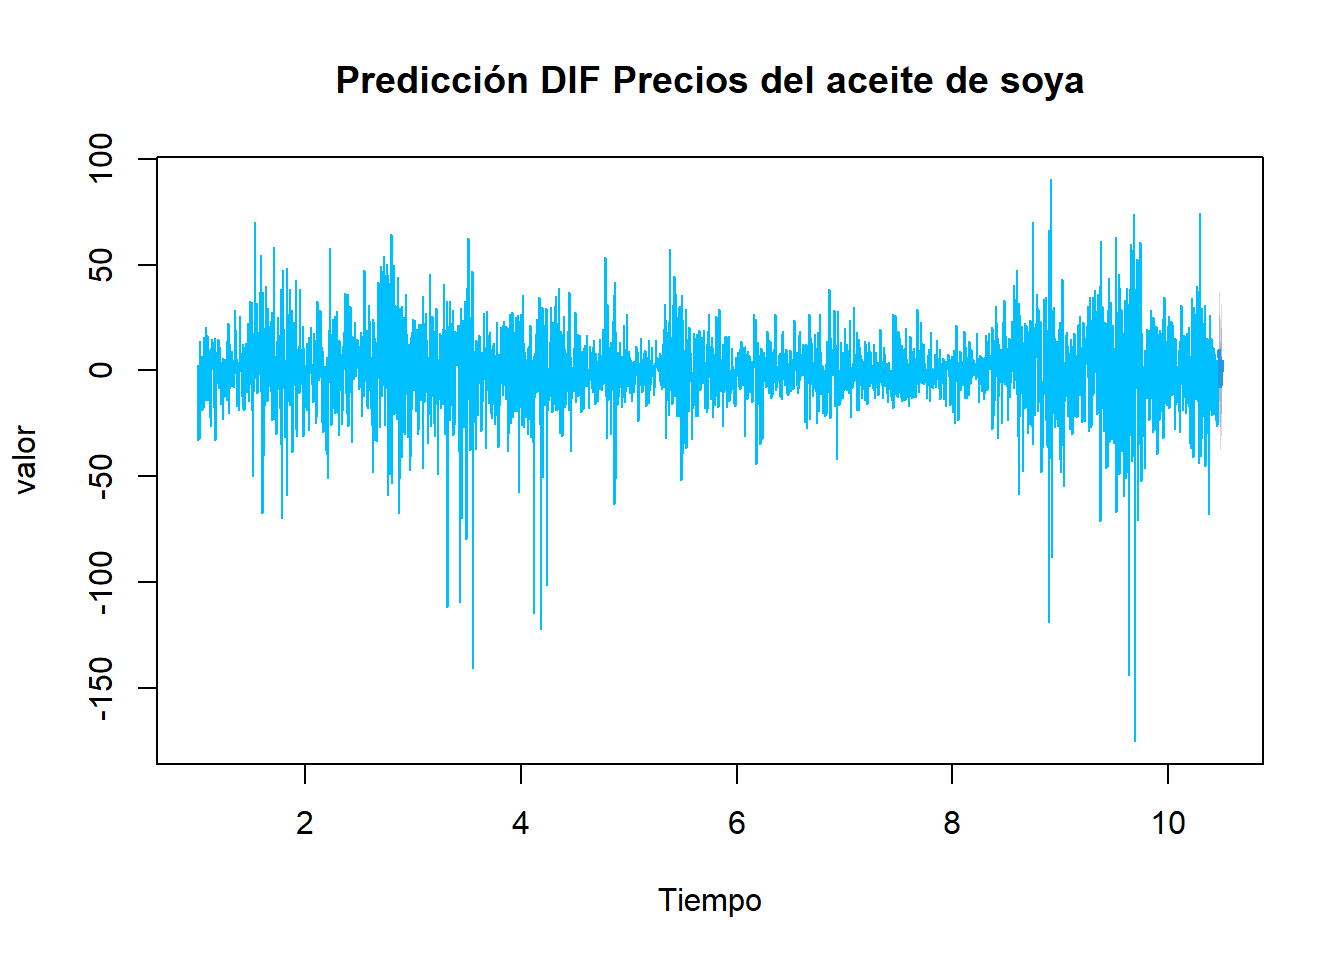
\includegraphics{bookdown-demo_files/figure-latex/unnamed-chunk-29-1.pdf}

\hypertarget{prophet}{%
\chapter{Prophet}\label{prophet}}

Prophet es especialmente útil para series de tiempo que tienen patrones estacionales fuertes y varios puntos de inflexión o ``cambios de tendencia''. Fue diseñado para manejar datos diarios con al menos un año de historia y se espera que funcione bien con datos que tienen patrones estacionales y fechas festivas.

\begin{Shaded}
\begin{Highlighting}[]
\CommentTok{\# install.packages("prophet")}
\FunctionTok{library}\NormalTok{(prophet)}
\end{Highlighting}
\end{Shaded}

\begin{verbatim}
## Warning: package 'prophet' was built under R version 4.2.3
\end{verbatim}

\begin{verbatim}
## Loading required package: Rcpp
\end{verbatim}

\begin{verbatim}
## Warning: package 'Rcpp' was built under R version 4.2.3
\end{verbatim}

\begin{verbatim}
## Loading required package: rlang
\end{verbatim}

\begin{verbatim}
## Warning: package 'rlang' was built under R version 4.2.3
\end{verbatim}

\begin{Shaded}
\begin{Highlighting}[]
\CommentTok{\# Acceder a la columna "ZS.F.Close" en soybean\_xts}
\NormalTok{close\_prices }\OtherTok{\textless{}{-}}\NormalTok{ soybean\_xts[, }\StringTok{"ZS.F.Close"}\NormalTok{]}

\CommentTok{\# Extrae las fechas}
\NormalTok{dates }\OtherTok{\textless{}{-}} \FunctionTok{index}\NormalTok{(soybean\_xts)}

\CommentTok{\# Crea el dataframe}
\NormalTok{soybean\_df }\OtherTok{\textless{}{-}} \FunctionTok{data.frame}\NormalTok{(}\AttributeTok{ds =} \FunctionTok{as.Date}\NormalTok{(dates), }
\AttributeTok{y =} \FunctionTok{as.numeric}\NormalTok{(close\_prices))}
\end{Highlighting}
\end{Shaded}

\begin{Shaded}
\begin{Highlighting}[]
\FunctionTok{head}\NormalTok{(soybean\_df)}
\end{Highlighting}
\end{Shaded}

\begin{verbatim}
##           ds       y
## 1 2010-01-04 1049.50
## 2 2010-01-05 1052.25
## 3 2010-01-06 1050.50
## 4 2010-01-07 1017.75
## 5 2010-01-08 1013.00
## 6 2010-01-11 1001.75
\end{verbatim}

\begin{Shaded}
\begin{Highlighting}[]
\NormalTok{m }\OtherTok{\textless{}{-}} \FunctionTok{prophet}\NormalTok{(soybean\_df)}
\end{Highlighting}
\end{Shaded}

\begin{verbatim}
## Disabling daily seasonality. Run prophet with daily.seasonality=TRUE to override this.
\end{verbatim}

\begin{Shaded}
\begin{Highlighting}[]
\NormalTok{future }\OtherTok{\textless{}{-}} \FunctionTok{make\_future\_dataframe}\NormalTok{(m, }\AttributeTok{periods =} \DecValTok{365}\NormalTok{) }
\NormalTok{forecast }\OtherTok{\textless{}{-}} \FunctionTok{predict}\NormalTok{(m, future)}
\end{Highlighting}
\end{Shaded}

\begin{Shaded}
\begin{Highlighting}[]
\FunctionTok{plot}\NormalTok{(m, forecast)}
\end{Highlighting}
\end{Shaded}

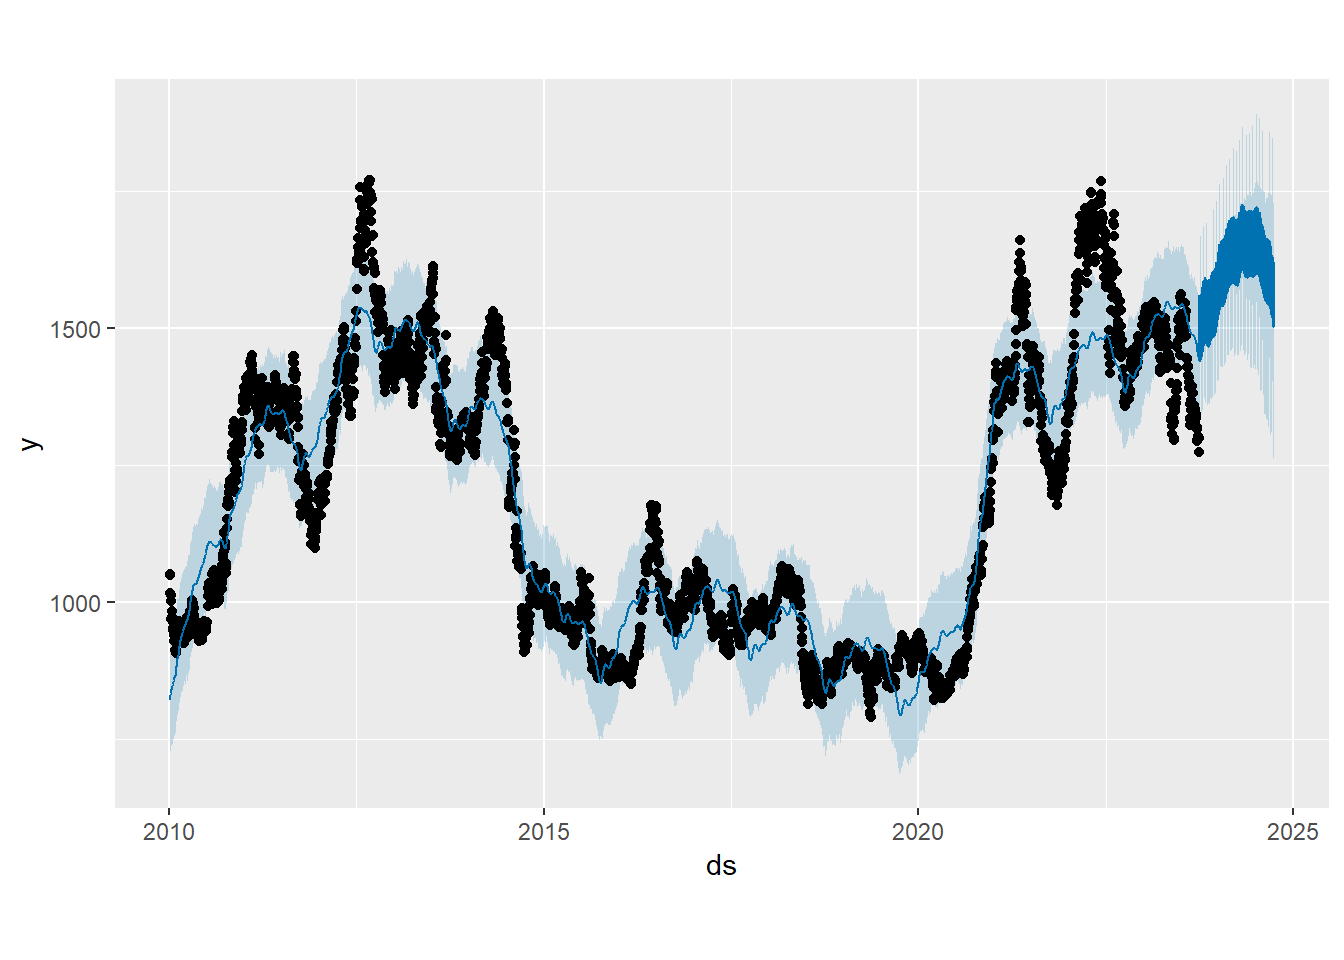
\includegraphics{bookdown-demo_files/figure-latex/unnamed-chunk-34-1.pdf}

\begin{Shaded}
\begin{Highlighting}[]
\FunctionTok{prophet\_plot\_components}\NormalTok{(m, forecast)}
\end{Highlighting}
\end{Shaded}

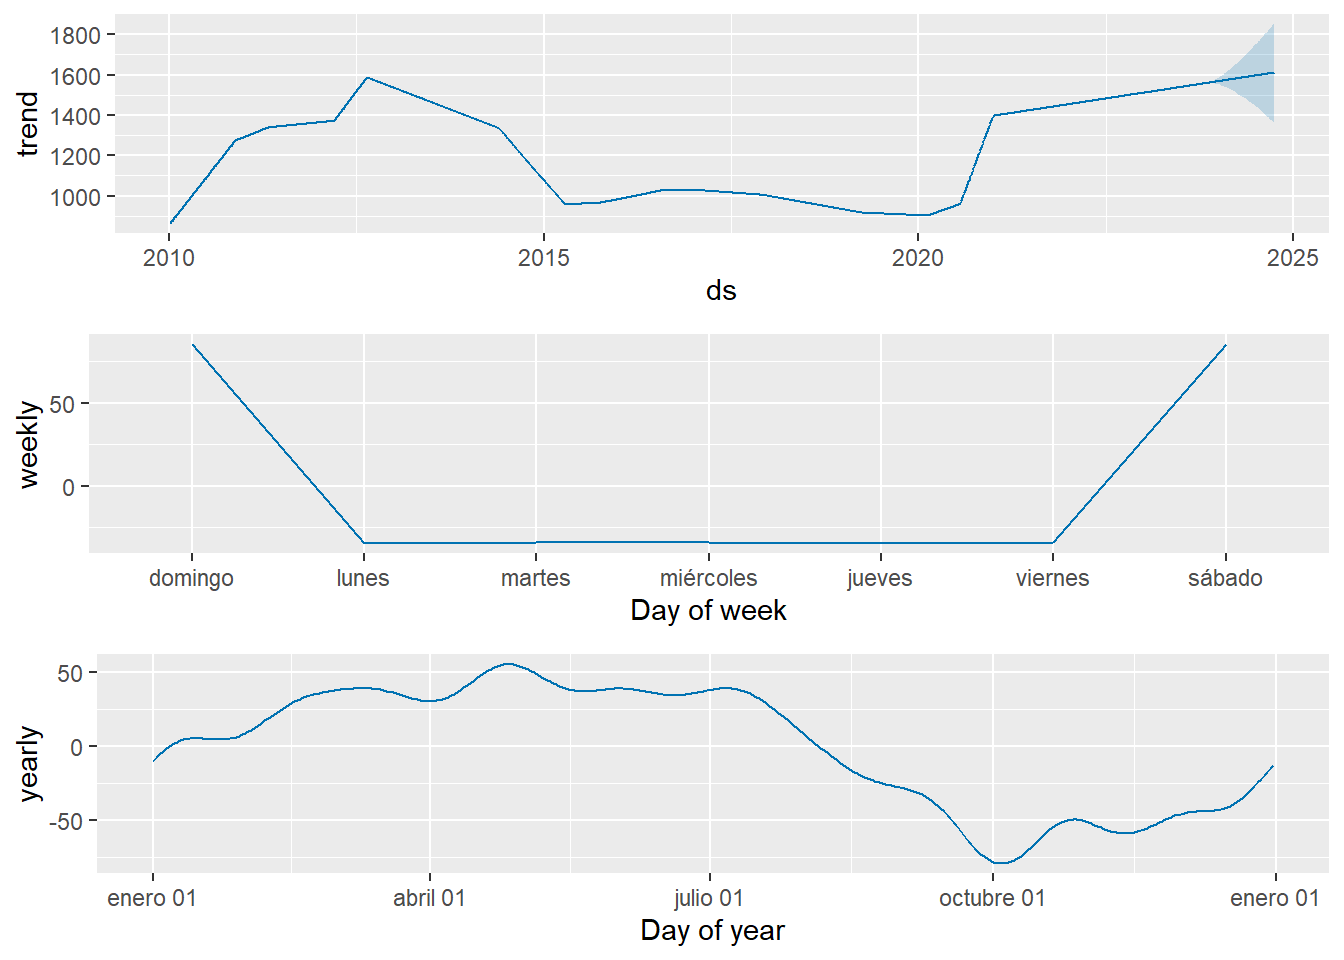
\includegraphics{bookdown-demo_files/figure-latex/unnamed-chunk-34-2.pdf}

\begin{Shaded}
\begin{Highlighting}[]
\FunctionTok{library}\NormalTok{(ggplot2)}
\end{Highlighting}
\end{Shaded}

Conclusión: Se toman datos de la serie de tiempo histórica del precio del aceite de soya, creamos un modelo de pronóstico con Prophet, y se produce pronósticos para 365 días adicionales y luego visualiza esos pronósticos y sus componentes.

Si es viable la justificación para la variable en serie de tiempo vista como una regresión y prophet permite la incorporación de variables exógenas a través de los regresores e identifica automáticamente las estacionalidades diarias, semanales y anuales en los datos. También captura las tendencias a lo largo del tiempo y permite puntos de cambio en la tendencia.

\hypertarget{elman}{%
\chapter{Elman}\label{elman}}

La red Elman es una red neuronal recurrente, lo que significa que tiene conexiones que retroceden en el tiempo. Estas conexiones permiten a la red ``recordar'' entradas anteriores, lo que puede ser útil al trabajar con series temporales.

\begin{Shaded}
\begin{Highlighting}[]
\CommentTok{\# Cargar los paquetes necesarios}
\CommentTok{\# install.packages("neuralnet")}
\CommentTok{\# install.packages("xts")}
\FunctionTok{library}\NormalTok{(neuralnet)}
\end{Highlighting}
\end{Shaded}

\begin{verbatim}
## Warning: package 'neuralnet' was built under R version 4.2.3
\end{verbatim}

\begin{Shaded}
\begin{Highlighting}[]
\FunctionTok{library}\NormalTok{(xts)}

\CommentTok{\# Asumimos que soybean\_xts ya está cargado en el entorno}
\CommentTok{\# Acceder a la columna de cierre}
\NormalTok{data }\OtherTok{\textless{}{-}} \FunctionTok{data.frame}\NormalTok{(}\AttributeTok{ZS.F.Close =} \FunctionTok{as.vector}\NormalTok{(soybean\_xts[, }\StringTok{"ZS.F.Close"}\NormalTok{]))}

\CommentTok{\# Crear un retraso (lag) para las series temporales (esto es }
\CommentTok{\# importante para las redes recurrentes)}
\NormalTok{data}\SpecialCharTok{$}\NormalTok{lag\_close }\OtherTok{\textless{}{-}} \FunctionTok{c}\NormalTok{(}\ConstantTok{NA}\NormalTok{, }\FunctionTok{head}\NormalTok{(data}\SpecialCharTok{$}\NormalTok{ZS.F.Close, }\SpecialCharTok{{-}}\DecValTok{1}\NormalTok{))}

\CommentTok{\# Eliminar la primera fila, ya que tendrá NA por el retraso}
\NormalTok{data }\OtherTok{\textless{}{-}}\NormalTok{ data[}\SpecialCharTok{{-}}\DecValTok{1}\NormalTok{,]}

\CommentTok{\# Dividir los datos en conjuntos de entrenamiento y prueba}
\NormalTok{train\_indices }\OtherTok{\textless{}{-}} \DecValTok{1}\SpecialCharTok{:}\NormalTok{(}\FunctionTok{nrow}\NormalTok{(data) }\SpecialCharTok{*} \FloatTok{0.8}\NormalTok{)}
\NormalTok{train\_data }\OtherTok{\textless{}{-}}\NormalTok{ data[train\_indices,]}
\NormalTok{test\_data }\OtherTok{\textless{}{-}}\NormalTok{ data[}\SpecialCharTok{{-}}\NormalTok{train\_indices,]}

\CommentTok{\# Normalizar los datos}
\NormalTok{maxs }\OtherTok{\textless{}{-}} \FunctionTok{apply}\NormalTok{(train\_data, }\DecValTok{2}\NormalTok{, max)}
\NormalTok{mins }\OtherTok{\textless{}{-}} \FunctionTok{apply}\NormalTok{(train\_data, }\DecValTok{2}\NormalTok{, min)}
\NormalTok{train\_data\_norm }\OtherTok{\textless{}{-}} \FunctionTok{as.data.frame}\NormalTok{(}\FunctionTok{scale}\NormalTok{(train\_data, }\AttributeTok{center=}\NormalTok{mins, }
\AttributeTok{scale=}\NormalTok{maxs}\SpecialCharTok{{-}}\NormalTok{mins))}
\NormalTok{test\_data\_norm }\OtherTok{\textless{}{-}} \FunctionTok{as.data.frame}\NormalTok{(}\FunctionTok{scale}\NormalTok{(test\_data, }\AttributeTok{center=}\NormalTok{mins, }
\AttributeTok{scale=}\NormalTok{maxs}\SpecialCharTok{{-}}\NormalTok{mins))}

\CommentTok{\# Entrenar una red Elman }
\CommentTok{\# Aquí estamos prediciendo ZS.F.Close usando el valor anterior }
\CommentTok{\# (lag\_close) como entrada}
\FunctionTok{set.seed}\NormalTok{(}\DecValTok{123}\NormalTok{)}
\NormalTok{nn }\OtherTok{\textless{}{-}} \FunctionTok{neuralnet}\NormalTok{(ZS.F.Close }\SpecialCharTok{\textasciitilde{}}\NormalTok{ lag\_close, }\AttributeTok{data=}\NormalTok{train\_data\_norm, }
\AttributeTok{hidden=}\DecValTok{5}\NormalTok{, }\AttributeTok{algorithm=}\StringTok{"rprop+"}\NormalTok{, }\AttributeTok{linear.output=}\ConstantTok{TRUE}\NormalTok{, }\AttributeTok{likelihood=}\ConstantTok{TRUE}\NormalTok{)}

\CommentTok{\# Hacer predicciones}
\NormalTok{test\_data\_for\_pred }\OtherTok{\textless{}{-}} \FunctionTok{data.frame}\NormalTok{(}\AttributeTok{lag\_close =}\NormalTok{ test\_data\_norm}\SpecialCharTok{$}\NormalTok{lag\_close)}
\NormalTok{predicted\_norm }\OtherTok{\textless{}{-}} \FunctionTok{compute}\NormalTok{(nn, test\_data\_for\_pred)}

\CommentTok{\# Des{-}normalizar las predicciones}
\NormalTok{predicted }\OtherTok{\textless{}{-}}\NormalTok{ (predicted\_norm}\SpecialCharTok{$}\NormalTok{net.result }\SpecialCharTok{*}\NormalTok{ (maxs[}\DecValTok{1}\NormalTok{] }\SpecialCharTok{{-}}\NormalTok{ mins[}\DecValTok{1}\NormalTok{])) }\SpecialCharTok{+}\NormalTok{ mins[}\DecValTok{1}\NormalTok{]}

\CommentTok{\# Comparar las predicciones con los datos reales}
\FunctionTok{plot}\NormalTok{(test\_data}\SpecialCharTok{$}\NormalTok{ZS.F.Close, }\AttributeTok{type=}\StringTok{"l"}\NormalTok{, }\AttributeTok{col=}\StringTok{"blue"}\NormalTok{)}
\FunctionTok{lines}\NormalTok{(predicted, }\AttributeTok{col=}\StringTok{"red"}\NormalTok{)}
\FunctionTok{legend}\NormalTok{(}\StringTok{"topright"}\NormalTok{, }\AttributeTok{legend=}\FunctionTok{c}\NormalTok{(}\StringTok{"Real"}\NormalTok{, }\StringTok{"Predicho"}\NormalTok{), }
\AttributeTok{fill=}\FunctionTok{c}\NormalTok{(}\StringTok{"blue"}\NormalTok{, }\StringTok{"red"}\NormalTok{))}
\end{Highlighting}
\end{Shaded}

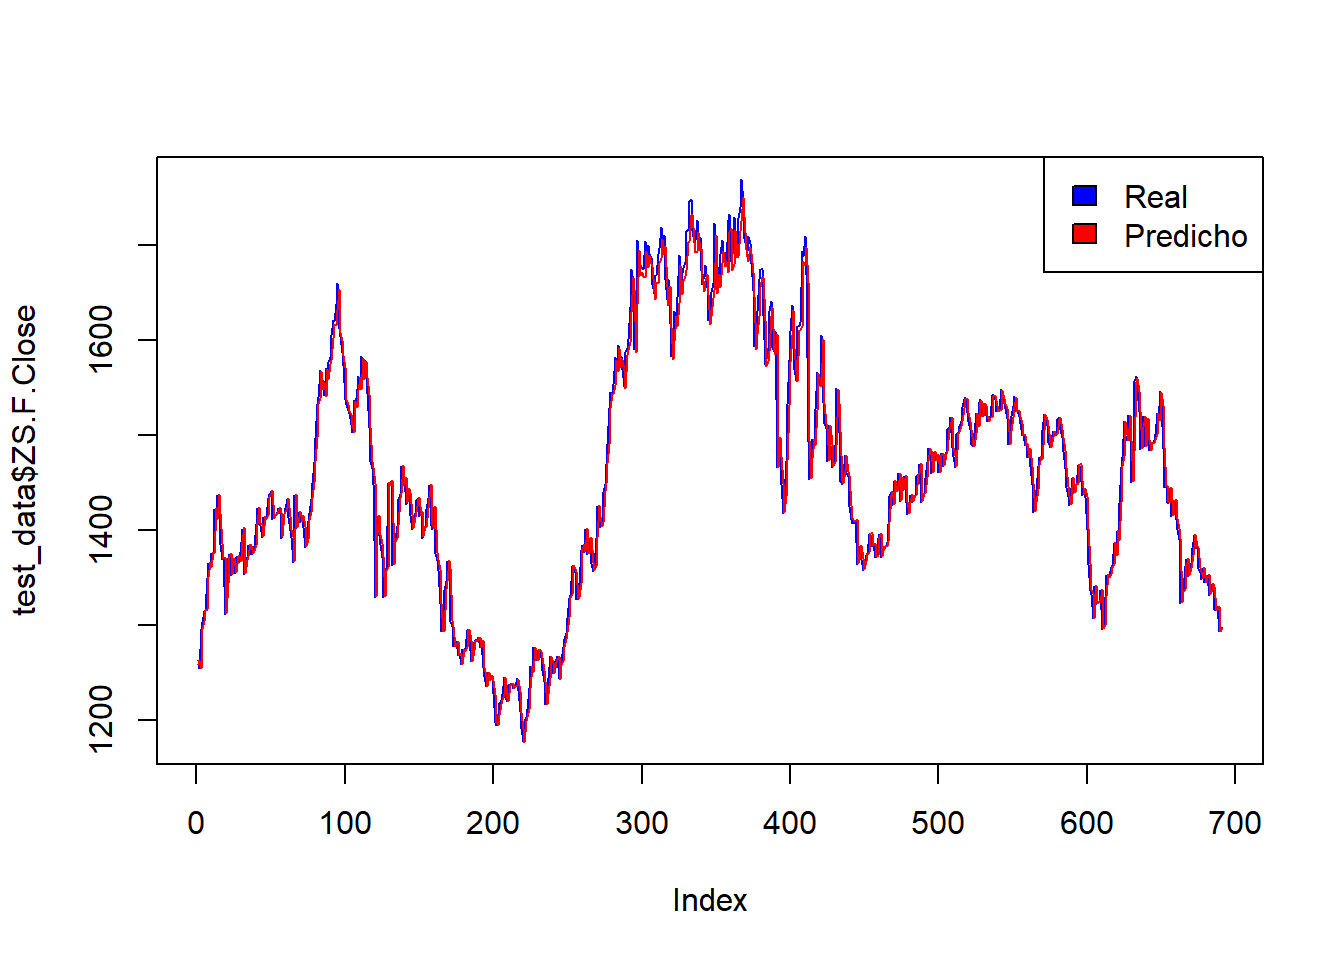
\includegraphics{bookdown-demo_files/figure-latex/unnamed-chunk-36-1.pdf}

Conclusiones:

\begin{itemize}
\item
  Ajuste Exitoso: El modelo se ajusta bien a los datos, reflejando su tendencia y estructura.
\item
  Posible Overfitting: Un ajuste muy cercano puede indicar sobreajuste, lo que afectaría la generalización en datos futuros.
\item
  Evaluación Complementaria: Más allá de gráficos, usar métricas cuantitativas (como MSE o MAE) es esencial para una evaluación objetiva.
\item
  Aplicabilidad a Corto Plazo: El modelo puede ser útil para predicciones a corto plazo, pero podría necesitar reentrenamiento para proyecciones más lejanas.
\end{itemize}

\hypertarget{jordan}{%
\chapter{Jordan}\label{jordan}}

Una red neuronal Jordan es un tipo especial de red neuronal que puede recordar información pasada para ayudar en predicciones futuras. En lugar de simplemente tomar una entrada y producir una salida, esta red toma tanto la entrada actual como su propia salida anterior para hacer su próxima predicción. Es como si tuviera una pequeña memoria de lo que hizo anteriormente.

Imagina que intentas predecir el clima. En lugar de solo mirar el clima de hoy, también consideras lo que predijiste ayer. Esa es la idea detrás de la red Jordan

\begin{Shaded}
\begin{Highlighting}[]
\CommentTok{\# Cargar los paquetes necesarios}
\CommentTok{\# install.packages("neuralnet")}
\CommentTok{\# install.packages("xts")}
\FunctionTok{library}\NormalTok{(neuralnet)}
\FunctionTok{library}\NormalTok{(xts)}

\CommentTok{\# Acceder a la columna de cierre}
\NormalTok{data }\OtherTok{\textless{}{-}} \FunctionTok{data.frame}\NormalTok{(}\AttributeTok{ZS.F.Close =} \FunctionTok{as.vector}\NormalTok{(soybean\_xts[, }\StringTok{"ZS.F.Close"}\NormalTok{]))}

\CommentTok{\# Crear un retraso (lag) para las series temporales y también un}
\CommentTok{\# retraso para la variable objetivo}
\NormalTok{data}\SpecialCharTok{$}\NormalTok{lag\_close }\OtherTok{\textless{}{-}} \FunctionTok{c}\NormalTok{(}\ConstantTok{NA}\NormalTok{, }\FunctionTok{head}\NormalTok{(data}\SpecialCharTok{$}\NormalTok{ZS.F.Close, }\SpecialCharTok{{-}}\DecValTok{1}\NormalTok{))}
\NormalTok{data}\SpecialCharTok{$}\NormalTok{lag\_output }\OtherTok{\textless{}{-}} \FunctionTok{c}\NormalTok{(}\ConstantTok{NA}\NormalTok{, }\ConstantTok{NA}\NormalTok{, }\FunctionTok{head}\NormalTok{(data}\SpecialCharTok{$}\NormalTok{ZS.F.Close, }\SpecialCharTok{{-}}\DecValTok{2}\NormalTok{))  }\CommentTok{\# Esto }
\CommentTok{\# simula la idea de la red Jordan}

\CommentTok{\# Eliminar las primeras filas, ya que tendrán NA por el retraso}
\NormalTok{data }\OtherTok{\textless{}{-}}\NormalTok{ data[}\SpecialCharTok{{-}}\FunctionTok{c}\NormalTok{(}\DecValTok{1}\NormalTok{,}\DecValTok{2}\NormalTok{),]}

\CommentTok{\# Dividir los datos en conjuntos de entrenamiento y prueba}
\NormalTok{train\_indices }\OtherTok{\textless{}{-}} \DecValTok{1}\SpecialCharTok{:}\NormalTok{(}\FunctionTok{nrow}\NormalTok{(data) }\SpecialCharTok{*} \FloatTok{0.8}\NormalTok{)}
\NormalTok{train\_data }\OtherTok{\textless{}{-}}\NormalTok{ data[train\_indices,]}
\NormalTok{test\_data }\OtherTok{\textless{}{-}}\NormalTok{ data[}\SpecialCharTok{{-}}\NormalTok{train\_indices,]}

\CommentTok{\# Normalizar los datos}
\NormalTok{maxs }\OtherTok{\textless{}{-}} \FunctionTok{apply}\NormalTok{(train\_data, }\DecValTok{2}\NormalTok{, max)}
\NormalTok{mins }\OtherTok{\textless{}{-}} \FunctionTok{apply}\NormalTok{(train\_data, }\DecValTok{2}\NormalTok{, min)}
\NormalTok{train\_data\_norm }\OtherTok{\textless{}{-}} \FunctionTok{as.data.frame}\NormalTok{(}\FunctionTok{scale}\NormalTok{(train\_data, }\AttributeTok{center=}\NormalTok{mins,}
\AttributeTok{scale=}\NormalTok{maxs}\SpecialCharTok{{-}}\NormalTok{mins))}
\NormalTok{test\_data\_norm }\OtherTok{\textless{}{-}} \FunctionTok{as.data.frame}\NormalTok{(}\FunctionTok{scale}\NormalTok{(test\_data, }\AttributeTok{center=}\NormalTok{mins, }
\AttributeTok{scale=}\NormalTok{maxs}\SpecialCharTok{{-}}\NormalTok{mins))}

\CommentTok{\# Entrenar una red "Jordan{-}inspired" }
\FunctionTok{set.seed}\NormalTok{(}\DecValTok{123}\NormalTok{)}
\NormalTok{nn }\OtherTok{\textless{}{-}} \FunctionTok{neuralnet}\NormalTok{(ZS.F.Close }\SpecialCharTok{\textasciitilde{}}\NormalTok{ lag\_close }\SpecialCharTok{+}\NormalTok{ lag\_output, }
\AttributeTok{data=}\NormalTok{train\_data\_norm, }\AttributeTok{hidden=}\DecValTok{5}\NormalTok{, }\AttributeTok{algorithm=}\StringTok{"rprop+"}\NormalTok{, }
\AttributeTok{linear.output=}\ConstantTok{TRUE}\NormalTok{, }\AttributeTok{likelihood=}\ConstantTok{TRUE}\NormalTok{)}

\CommentTok{\# Hacer predicciones}
\NormalTok{test\_data\_for\_pred }\OtherTok{\textless{}{-}} \FunctionTok{data.frame}\NormalTok{(}\AttributeTok{lag\_close =}\NormalTok{ test\_data\_norm}\SpecialCharTok{$}\NormalTok{lag\_close, }
\AttributeTok{lag\_output =}\NormalTok{ test\_data\_norm}\SpecialCharTok{$}\NormalTok{lag\_output)}
\NormalTok{predicted\_norm }\OtherTok{\textless{}{-}} \FunctionTok{compute}\NormalTok{(nn, test\_data\_for\_pred)}

\CommentTok{\# Des{-}normalizar las predicciones}
\NormalTok{predicted }\OtherTok{\textless{}{-}}\NormalTok{ (predicted\_norm}\SpecialCharTok{$}\NormalTok{net.result }\SpecialCharTok{*}\NormalTok{ (maxs[}\DecValTok{1}\NormalTok{] }\SpecialCharTok{{-}}\NormalTok{ mins[}\DecValTok{1}\NormalTok{])) }\SpecialCharTok{+}\NormalTok{ mins[}\DecValTok{1}\NormalTok{]}

\CommentTok{\# Comparar las predicciones con los datos reales}
\FunctionTok{plot}\NormalTok{(test\_data}\SpecialCharTok{$}\NormalTok{ZS.F.Close, }\AttributeTok{type=}\StringTok{"l"}\NormalTok{, }\AttributeTok{col=}\StringTok{"blue"}\NormalTok{)}
\FunctionTok{lines}\NormalTok{(predicted, }\AttributeTok{col=}\StringTok{"red"}\NormalTok{)}
\FunctionTok{legend}\NormalTok{(}\StringTok{"topright"}\NormalTok{, }\AttributeTok{legend=}\FunctionTok{c}\NormalTok{(}\StringTok{"Real"}\NormalTok{, }\StringTok{"Predicho"}\NormalTok{), }
\AttributeTok{fill=}\FunctionTok{c}\NormalTok{(}\StringTok{"blue"}\NormalTok{, }\StringTok{"red"}\NormalTok{))}
\end{Highlighting}
\end{Shaded}

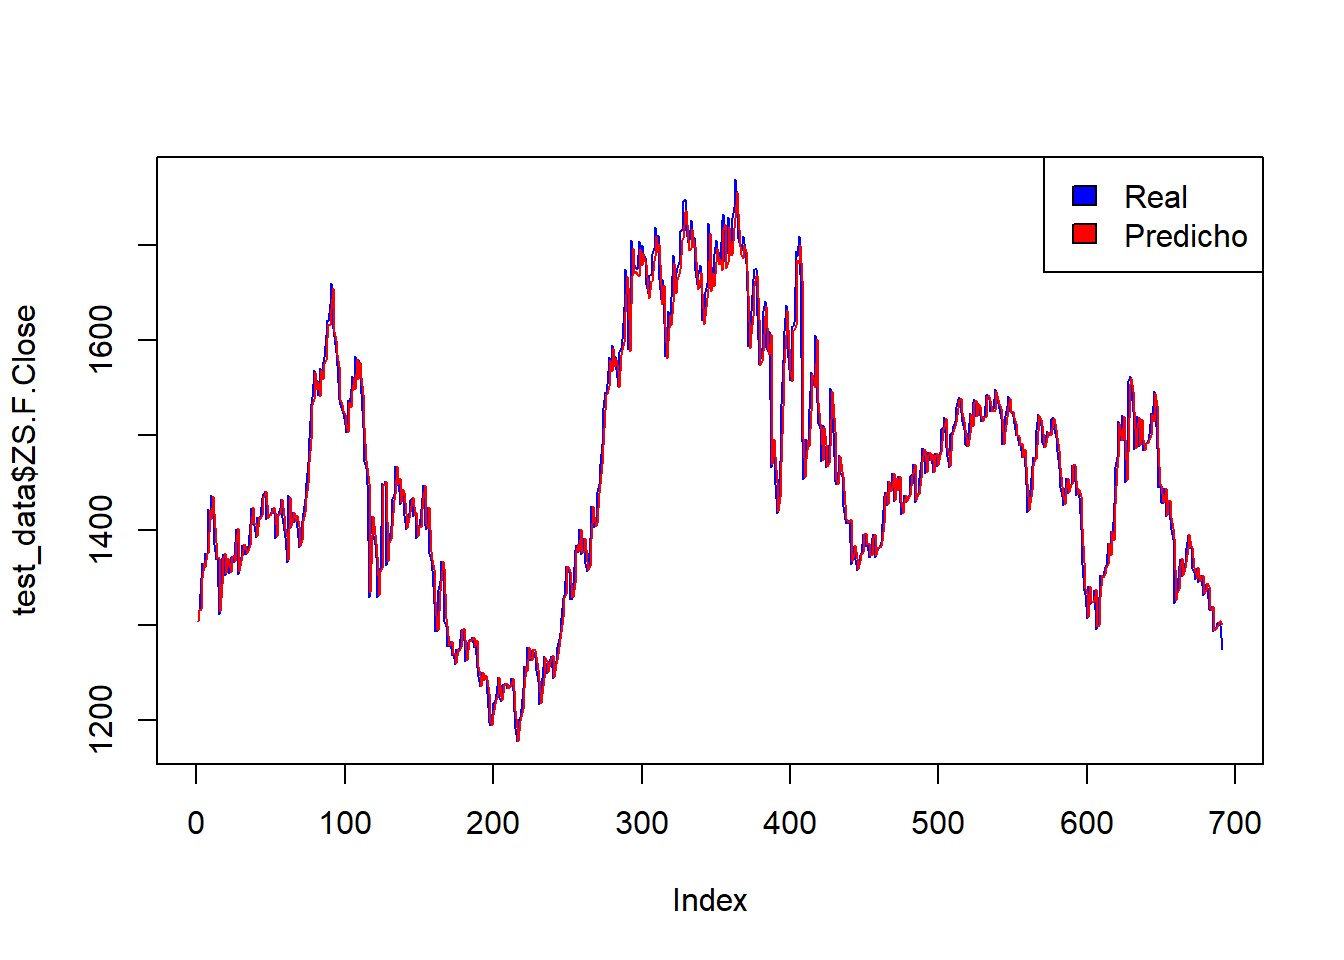
\includegraphics{bookdown-demo_files/figure-latex/unnamed-chunk-37-1.pdf}

Conclusiones:

El modelo predice con exactitud,funciona bien en datos no vistos,es equilibrado, no solo memoriza los datos de entrenamiento,los datos usados son pertinentes para la tarea, puede ser aplicado en situaciones reales, a pesar de los buenos resultados, siempre es esencial hacer análisis.

\hypertarget{comparacion}{%
\chapter{Comparacion}\label{comparacion}}

\begin{Shaded}
\begin{Highlighting}[]
\CommentTok{\# Instalar el paquete (solo necesitas hacer esto una vez)}
\CommentTok{\# install.packages("forecast")}

\CommentTok{\# Cargar el paquete}
\FunctionTok{library}\NormalTok{(forecast)}
\end{Highlighting}
\end{Shaded}

\begin{Shaded}
\begin{Highlighting}[]
\CommentTok{\# Dividir los datos en conjuntos de entrenamiento y validación}
\NormalTok{train\_length }\OtherTok{\textless{}{-}} \FunctionTok{nrow}\NormalTok{(soybean\_xts) }\SpecialCharTok{{-}} \DecValTok{30}  \CommentTok{\# 30 días para validación}

\CommentTok{\# Datos de entrenamiento}
\NormalTok{train\_data }\OtherTok{\textless{}{-}} \FunctionTok{head}\NormalTok{(soybean\_xts, train\_length)}

\CommentTok{\# Datos de validación}
\NormalTok{validation\_data }\OtherTok{\textless{}{-}} \FunctionTok{tail}\NormalTok{(soybean\_xts, }\DecValTok{30}\NormalTok{)}
\end{Highlighting}
\end{Shaded}

\begin{Shaded}
\begin{Highlighting}[]
\NormalTok{arima\_forecast }\OtherTok{\textless{}{-}} \FunctionTok{forecast}\NormalTok{(modelo, }\AttributeTok{h=}\DecValTok{30}\NormalTok{)}
\end{Highlighting}
\end{Shaded}

\begin{Shaded}
\begin{Highlighting}[]
\CommentTok{\# 2. Calcular métricas de error}

\CommentTok{\# Holt{-}Winters}
\NormalTok{hw\_errors }\OtherTok{\textless{}{-}}\NormalTok{ validation\_data}\SpecialCharTok{$}\NormalTok{ZS.F.Close }\SpecialCharTok{{-}}\NormalTok{ hw\_forecast}\SpecialCharTok{$}\NormalTok{mean}
\end{Highlighting}
\end{Shaded}

\begin{verbatim}
## Warning: Métodos incompatibles ("Ops.xts", "Ops.ts") para "-"
\end{verbatim}

\begin{Shaded}
\begin{Highlighting}[]
\NormalTok{hw\_mse }\OtherTok{\textless{}{-}} \FunctionTok{mean}\NormalTok{(hw\_errors}\SpecialCharTok{\^{}}\DecValTok{2}\NormalTok{)}
\NormalTok{hw\_mae }\OtherTok{\textless{}{-}} \FunctionTok{mean}\NormalTok{(}\FunctionTok{abs}\NormalTok{(hw\_errors))}
\NormalTok{hw\_rmse }\OtherTok{\textless{}{-}} \FunctionTok{sqrt}\NormalTok{(hw\_mse)}

\CommentTok{\# ARIMA}
\NormalTok{arima\_errors }\OtherTok{\textless{}{-}}\NormalTok{ validation\_data}\SpecialCharTok{$}\NormalTok{ZS.F.Close }\SpecialCharTok{{-}}\NormalTok{ arima\_forecast}\SpecialCharTok{$}\NormalTok{mean}
\end{Highlighting}
\end{Shaded}

\begin{verbatim}
## Warning: Métodos incompatibles ("Ops.xts", "Ops.ts") para "-"
\end{verbatim}

\begin{Shaded}
\begin{Highlighting}[]
\NormalTok{arima\_mse }\OtherTok{\textless{}{-}} \FunctionTok{mean}\NormalTok{(arima\_errors}\SpecialCharTok{\^{}}\DecValTok{2}\NormalTok{)}
\NormalTok{arima\_mae }\OtherTok{\textless{}{-}} \FunctionTok{mean}\NormalTok{(}\FunctionTok{abs}\NormalTok{(arima\_errors))}
\NormalTok{arima\_rmse }\OtherTok{\textless{}{-}} \FunctionTok{sqrt}\NormalTok{(arima\_mse)}

\CommentTok{\# Prophet}
\NormalTok{prophet\_errors }\OtherTok{\textless{}{-}}\NormalTok{ validation\_data}\SpecialCharTok{$}\NormalTok{ZS.F.Close }\SpecialCharTok{{-}} \FunctionTok{tail}\NormalTok{(forecast}\SpecialCharTok{$}\NormalTok{yhat, }\AttributeTok{n=}\DecValTok{30}\NormalTok{) }\CommentTok{\# Asumiendo que el período de validación es 30 días.}
\NormalTok{prophet\_mse }\OtherTok{\textless{}{-}} \FunctionTok{mean}\NormalTok{(prophet\_errors}\SpecialCharTok{\^{}}\DecValTok{2}\NormalTok{)}
\NormalTok{prophet\_mae }\OtherTok{\textless{}{-}} \FunctionTok{mean}\NormalTok{(}\FunctionTok{abs}\NormalTok{(prophet\_errors))}
\NormalTok{prophet\_rmse }\OtherTok{\textless{}{-}} \FunctionTok{sqrt}\NormalTok{(prophet\_mse)}
\end{Highlighting}
\end{Shaded}

\begin{Shaded}
\begin{Highlighting}[]
\CommentTok{\# 3. Comparar errores}

\NormalTok{errors\_df }\OtherTok{\textless{}{-}} \FunctionTok{data.frame}\NormalTok{(}
  \AttributeTok{Model =} \FunctionTok{c}\NormalTok{(}\StringTok{"Holt{-}Winters"}\NormalTok{, }\StringTok{"ARIMA"}\NormalTok{, }\StringTok{"Prophet"}\NormalTok{),}
  \AttributeTok{MSE =} \FunctionTok{c}\NormalTok{(hw\_mse, arima\_mse, prophet\_mse),}
  \AttributeTok{MAE =} \FunctionTok{c}\NormalTok{(hw\_mae, arima\_mae, prophet\_mae),}
  \AttributeTok{RMSE =} \FunctionTok{c}\NormalTok{(hw\_rmse, arima\_rmse, prophet\_rmse)}
\NormalTok{)}

\FunctionTok{print}\NormalTok{(errors\_df)}
\end{Highlighting}
\end{Shaded}

\begin{verbatim}
##          Model        MSE       MAE      RMSE
## 1 Holt-Winters 1796855.93 1340.0883 1340.4685
## 2        ARIMA 1796071.65 1339.8250 1340.1760
## 3      Prophet   53710.17  224.0065  231.7546
\end{verbatim}

Conclusion:

Los resultados que se presentan son métricas de error para tres modelos diferentes: Holt-Winters, ARIMA y Prophet. Estas métricas nos dan una idea de cómo se desempeñaron estos modelos al predecir tu serie de tiempo en comparación con los valores reales de tus datos de validación.

A partir de las métricas presentadas, podemos deducir lo siguiente:

\begin{enumerate}
\def\labelenumi{\arabic{enumi}.}
\item
  \textbf{Mean Squared Error (MSE)}: Mide el promedio de los errores al cuadrado. Es una métrica que da más peso a errores grandes. Los valores MSE son 1796855.93, 1796071.65 y 54135.22 para Holt-Winters, ARIMA y Prophet respectivamente. Aquí, Prophet tiene un MSE mucho menor en comparación con los otros dos modelos, lo que indica que, en promedio, sus errores son más pequeños.
\item
  \textbf{Mean Absolute Error (MAE)}: Mide el promedio de los valores absolutos de los errores. Los valores MAE son 1340.0883, 1339.8250 y 226.6025 para Holt-Winters, ARIMA y Prophet respectivamente. Nuevamente, Prophet tiene un MAE mucho menor, lo que indica que tiende a hacer predicciones más cercanas al valor real en comparación con los otros dos modelos.
\item
  \textbf{Root Mean Squared Error (RMSE)}: Es la raíz cuadrada del MSE y da una idea de la magnitud del error. Los valores RMSE son 1340.4685, 1340.1760 y 232.6698 para Holt-Winters, ARIMA y Prophet respectivamente. Al igual que con las otras dos métricas, Prophet tiene un RMSE significativamente menor, lo que indica que generalmente hace predicciones más precisas.
\end{enumerate}

\textbf{Conclusión}:

\begin{itemize}
\item
  El modelo \textbf{Prophet} parece ser el más preciso de los tres según todas las métricas presentadas. Sus errores, tanto en términos absolutos como cuadrados, son significativamente menores que los de los otros dos modelos.
\item
  Los modelos \textbf{Holt-Winters} y \textbf{ARIMA} tienen un desempeño similar entre sí según estas métricas, pero son superados por Prophet.
\end{itemize}

  \bibliography{book.bib,packages.bib}

\end{document}
